\documentclass[12pt, a4paper]{article}
\usepackage[utf8]{inputenc}
\usepackage[russian]{babel}
\usepackage[T2A]{fontenc}
\usepackage{amsfonts}
\usepackage{amsmath}
\usepackage{indentfirst}
\usepackage{amsthm}
\usepackage{algorithm,algpseudocode}
\usepackage{float} 
\usepackage{cmap}
\usepackage{multirow}
\usepackage[hidelinks]{hyperref}
\DeclareMathOperator*{\argmin}{argmin}
\newtheorem{lemma}{Лемма}[section]
\newtheorem{state}{Утверждение}[section]

\usepackage[left=2cm,right=1.5cm,top=2cm,bottom=2cm]{geometry}
\linespread{1.25}

\usepackage{graphicx}
\graphicspath{{pictures/}}
\DeclareGraphicsExtensions{.pdf,.png,.jpg}

\begin{document}
	\pagestyle{empty}
	
	\begin{center}
		ФЕДЕРАЛЬНОЕ ГОСУДАРСТВЕННОЕ БЮДЖЕТНОЕ ОБРАЗОВАТЕЛЬНОЕ\\
		УЧРЕЖДЕНИЕ ВЫСШЕГО ОБРАЗОВАНИЯ\\
		<<МОСКОВСКИЙ ГОСУДАРСТВЕННЫЙ УНИВЕРСИТЕТ\\
		имени М.\,В.~ЛОМОНОСОВА>>
	\end{center}
	\vspace{4pt}
	\begin{center}
		МЕХАНИКО-МАТЕМАТИЧЕСКИЙ ФАКУЛЬТЕТ
	\end{center}
	\vspace{4pt}
	\begin{center}
		КАФЕДРА ВЫЧИСЛИТЕЛЬНОЙ МАТЕМАТИКИ
	\end{center}
	\vspace{1cm}
	\begin{center}
		ВЫПУСКНАЯ КВАЛИФИКАЦИОННАЯ РАБОТА\\
		специалиста
	\end{center}
	
	\begin{center}
		\textbf{ПОСТРОЕНИЕ ОПТИМАЛЬНОГО МАРШРУТА \\
			ПРИ ЗАДАННОЙ МОДЕЛИ ДВИЖЕНИЯ ДРУГИХ \\
			УЧАСТНИКОВ ТРАНСПОРТНОЙ СЕТИ}
	\end{center}
	\vspace{1cm}
	\begin{center}
		\begin{tabular}{p{9cm} l}
			& Выполнил студент $610$ группы\\
			& Разумова Любовь Евгеньевна\\
			& $\phantom{C_n^k=C_n^{n-k}}$\\
			& $\underline{\phantom{\int\limits_a^bf(x)dx=F(b)-F(a)}}$\\
			& подпись студента\\
			& $\phantom{\int\limits_f(z)dz=0}$\\
			& Научный руководитель:\\
			& кандидат физико-математических наук \\
			& Афонин Сергей Александрович\\
			& $\phantom{C_n^k=C_n^{n-k}}$\\
			& $\underline{\phantom{\int\limits_a^bf(x)dx=F(b)-F(a)}}$\\
			& подпись научного руководителя\\
		\end{tabular}
	\end{center}
	\vspace{1cm}
	\begin{center}
		Москва\\
		$2022$
	\end{center}
	
	\newpage
	\pagestyle{plain}
	\tableofcontents{}
	
	\newpage	
	
	\section*{Введение}
	
	В данной работе рассматривается задача нахождения наилучшего в смысле временных затрат пути с учетом движения фиксированного количества участников по заданным маршрутам в рамках некоторой модели движения. Под моделью движения понимается некий набор правил, которые задают скоростной режим участника движения в зависимости от его взаимодействия с другими автомобильными транспортными средствами (АТС). Маршруты участников могут пересекаться, что приводит к изменению скорости участников и образованию заторов. Целью работы является проложение оптимального маршрута в условиях возможности возникновения пробок на вариации подходящих путей.
	
	%Одной из подзадач является разработка таких правил, которые были бы близки к естсвественному характеру взаимодействия автомобильных  траснспортных средств (АТС).
	%в условиях ограниченности модели дорожной системы.
	
	\if 0
	В данной работе рассматривается задача нахождения наилучшего в каком-то смысле пути с учетом движения фиксированного количества участников по заданным ранее маршрутам в условиях ограниченности модели дорожной системы. Новый построенный маршрут должен отвечать выбранному критерию оптимальности среди всевозможных путей на всем временном промежутке, но не обязательно в каждый момент времени. Знание маршрутов изначальных участников помогает определить плотность автомобильного потока на конкретных отрезках пути. Рассматриваемая модель приближена к реальной дорожной системе городов, поэтому на всех ее участках наложены ограничения по вместимости участников и скорости их движения. Такие ограничения влияют на показатели маршрутов участников, такие как итоговое время движения и длину пути. 
	\fi
	
	В наше время задачи на транспортную тематику приобретают особую актуальность, в том числе и задача маршрутизации. Сложно найти человека, который в целях сбережения личного времени не пользуется какой-нибудь системой навигации, не говоря уже о сервисах такси, для которых крайне важно минимизировать временные затраты в пути. Однако данная задача решается построением оптмального маршрута с учетом картины заторов на момент составления этого маршрута. Образование заторов --- часто непредсказуемое явление, и пробка может появиться прямо перед нами на участке пути, который при построении маршрута был свободен. Несмотря на то, что время и место заторов сложно предугадать, задачей их прогнозирования занимаются уже долгое время.
	% Тема актуальна и в наше время, так как она помогает решать проблему возникновения пробок на дорогах, а также призвана упростить водителям выбор маршрута, который займет у них наименьшее время. 
	%Задача имеет практический характер... Проблема пробок в Москве стоит очень остро, ученые решают ее не первый год..
	
	%Помимо систем навигации прогнозы загруженности используются для автоматического управления дорожным движением в некоторых городах. Первые прототипы, в которых были применены прогнозы, появились появились в 1998 году в США. А первое пилотное использование системы, «заглядывающей в будущее», началось в 2006 году в Сингапуре в целях заблаговременного предупреждения водителей о дорожных условиях впереди и ценах, взимаемых за пробки в данный момент. 
	Среди наших соотечественников задачей прогнозирования занимаются разработчики Яндекс.Пробок. Программисты собирают информацию по трекам движения автомобилей, осуществляют привязку треков к ребрам графа дорожной сети, вычисляют некоторую усредненную скорость на отдельных участках, рисуют карту прогноза дорожной ситуации на ближайший час и в связи с этим предлагают оптимальный по времени путь, а также еще пару альтернативных маршрутов. Сложность сбора информации и построения треков движения состоит в том, что, во-первых, не все пользуются сервисами Яндекса при построении своего маршрута, и во-вторых, в данных постоянно возникают лишние шумы, что приводит к выбросам на графиках, и с таким качеством информации работать очень сложно. Также стоит отметить, что разработчики Яндекс.Пробок используют статистические методы и машинное обучение в качестве инструмента для решения своих задач.
	
	Мы рассматриваем более прозрачную и простую модель, когда все маршруты изначально проложены и известны, и они не меняются с течением времени. Такой уровень информированности о движении участников вряд ли достижим в реальной жизни, но это не умаляет значимости и важности поставленной нами задачи. Путем моделирования движения можно получить более точные результаты, идеи в дальнейшем могут развиваться и открывать новые возможности для более широкой задачи, например, как у Яндекса. 
	%Стоит отметить, что на конференции Yet another Conference в 2012 году разработчики впервые поделились результатами о применении машинного обучения в прогнозировании пробок. До этого пользователи могли пользоваться только картой пробок на текущий момент и историческим прогнозом на основе статистики.  
	% Также стоит отметить, что разработчики Яндекс.Пробок используют статистические методы и машинное обучение в качестве инструмента для решения своих задач, мы же подойдем к вопросу с другой стороны и применим другие алгоритмы.
	
	
	Важную роль в задачах маршрутизации играет представление правил движения АТС с помощью формальной математической модели.
	%формальные математические модели, описывающие правила движения АТС. 
	Она должна быть подобрана на основе имеющихся данных.
	%Олно и то же движение транспортного потока можно описать разными математическими моделями, поэтому выбор модели очень важен?
	%Одна и та же дорожная ситуация в разных моделях будет
	%Отдельное внимание стоит уделить построению математической модели для описания движения АТС. 
	Существует множество различных моделей движения, например, в модели Лайтхилла–Уизема (Уитема)–Ричардса (LWR) \cite{hydro_1}, \cite{hydro_2} однополосный транспортный поток рассматривается как поток одномерной сжимаемой жидкости. Модель LWR была первой среди гидродинамических. Теория развивалась и появлялись новые модели, такие как модель Танака \cite{Tanaka} --- LWR-модель, где плотность потока зависит от некоторой дистанции видимости, зависящей от скорости потока. В микроскопической модели Ньюэлла \cite{Newwell} постулируется, что для каждого водителя существует безопасная скорость движения, зависящая от дистанции до лидера. 
	В своей работе мы позаимствовали деление моделей движения на макро- и микроскопические \cite{book} и разработали свои модели взаимодействия участников движения.
	
	
	Задачи, которые мы ставили перед собой в рамках выбранной темы дипломной работы: формальная постановка задачи, анализ полученных ранее результатов в этой теме, разработка модели движения, которая была бы близка к естественному характеру взаимодействия АТС, исследование применимости различных алгоритмов к решению поставленной задачи. Методом исследования задачи оптимизации является моделирование движения.
	
	%Основа нашей задачи - нахождение наилучшего пути в условиях изменчивости плотности и скорости дорожного потока на участках в заисимости от времени.
	
	В первом разделе введем определение модели движения как некоторого автомата и в этих терминах опишем поставленную задачу. Во втором разделе будет представлена классификация моделей движения с примерами. Далее мы опишем процесс моделирования произвольной дорожной ситуации. Четвертый раздел посвящен описанию алгоритмов и исследованию их применимости. В завершение получим результаты тестирования алгоритмов и сделаем выводы.
	
	
	
	
	\newpage
	\section{Постановка задачи}
	
	Пусть задан ориентированный \textit{граф дорожной сети} $ G (V, E, l)$ таким образом, что вершины $V$ осуществляют роль перекрестков, а ребра $E$ --- роль дорог. Каждое ребро имеет длину, т.е. задана функция $l : E \rightarrow \mathbb {R} $. Также мы говорим, что задана некоторая модель движения.
	%Формализуем понятие модели движения, упомянутое в постановке задачи.  Обратимся к теории автоматов и с ее помощью попробуем описать правила движения АТС.
	Обратимся к теории автоматов, чтобы попробовать формализовать подразумеваемые под этим понятием правила движения АТС. Аналогичный подход использовали К.\,Нагель и М.\,Шрекенберг \cite{automat_baza}. В своей работе авторы рассматривают модель клеточных автоматов, которая предполагает разбиение дорог на клетки и использование дискретного времени. Эта идея нашла применение в описании движения физических частиц \cite{automat_phyz}, а также в исследовании пробок на дорогах \cite{automat_jam}. Мы же не будем ограничиваться клеточными автоматами и опишем случай непрерывного движения.
	
	\textit{Моделью движения} АТС назовем $M = \left(n, G, S, \{s^{0}_i\} _{i=1}^n, \{F_i\}_{i = 1}^n, \{t_i\}_{i = 1}^n, \{\varphi_i\}_{i = 1}^n \right)$, где $n$ --- количество участников движения, $G$ --- граф дорожной сети, $S$ --- множество состояний, которые могут принимать участники, $s^0_i \in S$ --- начальное состояние участника $i$, $F_i \subset S$ --- множество заключительных состояний участника $i$, $t_i: S^n \rightarrow R_{\ge0}$ --- функция критического момента движения участника $i$, $\varphi_i: S^n \times \mathbb{R}_{\ge 0} \rightarrow S$ --- функция перехода состояния $i$-ого участника в некоторый момент времени $t$. 
	
	Выбор множества $S$ зависит от правил движения, которые мы хотим описать. Например, правила движения могут учитывать положение на графе $(e, x) \in E \times [0; 1]$, скорость $v \in \mathbb{R}$ участника и время в пути $t \in \mathbb{R}$. В таком случае считаем $S = E \times [0; 1] \times \mathbb{R}^2$.
	Подразумевается, что состояния можно разбить на классы, например <<свободное движение>>, <<ожидание>>, <<прибытие>>, <<торможение>>, <<ускорение>> и тд. Функция $t_i$ описывает время, когда участнику необходимо совершить переход из текущего состояния в состояние другого класса. 
	Считаем, что, попав в заключительное состояние, мы не можем его покинуть:
	$$\varphi_i (s_1, \dots, s_i, \dots, s_n, t) = s_i, \text{ } s_1, \dots, s_n \in S, \text{ } s_i \in F_i, \text{ } \forall t \in \mathbb{R}_{\ge 0}.$$
	
	Модель движения АТС можно изобразить некоторой диаграммой, описывающей переходы между классами для каждого участника. Диаграмма представляет собой ориентированный граф, где вершины --- классы состояний, а ребра являются переходами в другое состояние. Метка на ребре --- условие перехода, который осуществляется, если $t =  t_i(s_1, \dots, s_n)$ для некоторого $s_i$ из класса состояний. Непомеченные ребра соответствуют условию $t < t_i(s_1, \dots, s_n)$:
	$$\varphi_i (s_1, \dots, s_n, t) = s_i, \text{ } s_1, \dots, s_n \in S, \text{ } 0 \le t < t_i(s_1, \dots, s_n).$$
	Например, правила движения, в которых поведение участника зависит от расстояния до впереди идущего участника, могут быть заданы следующей диаграммой (см. рис. \ref{ris:example_diag}):
	\begin{figure}[H]
		\centering
		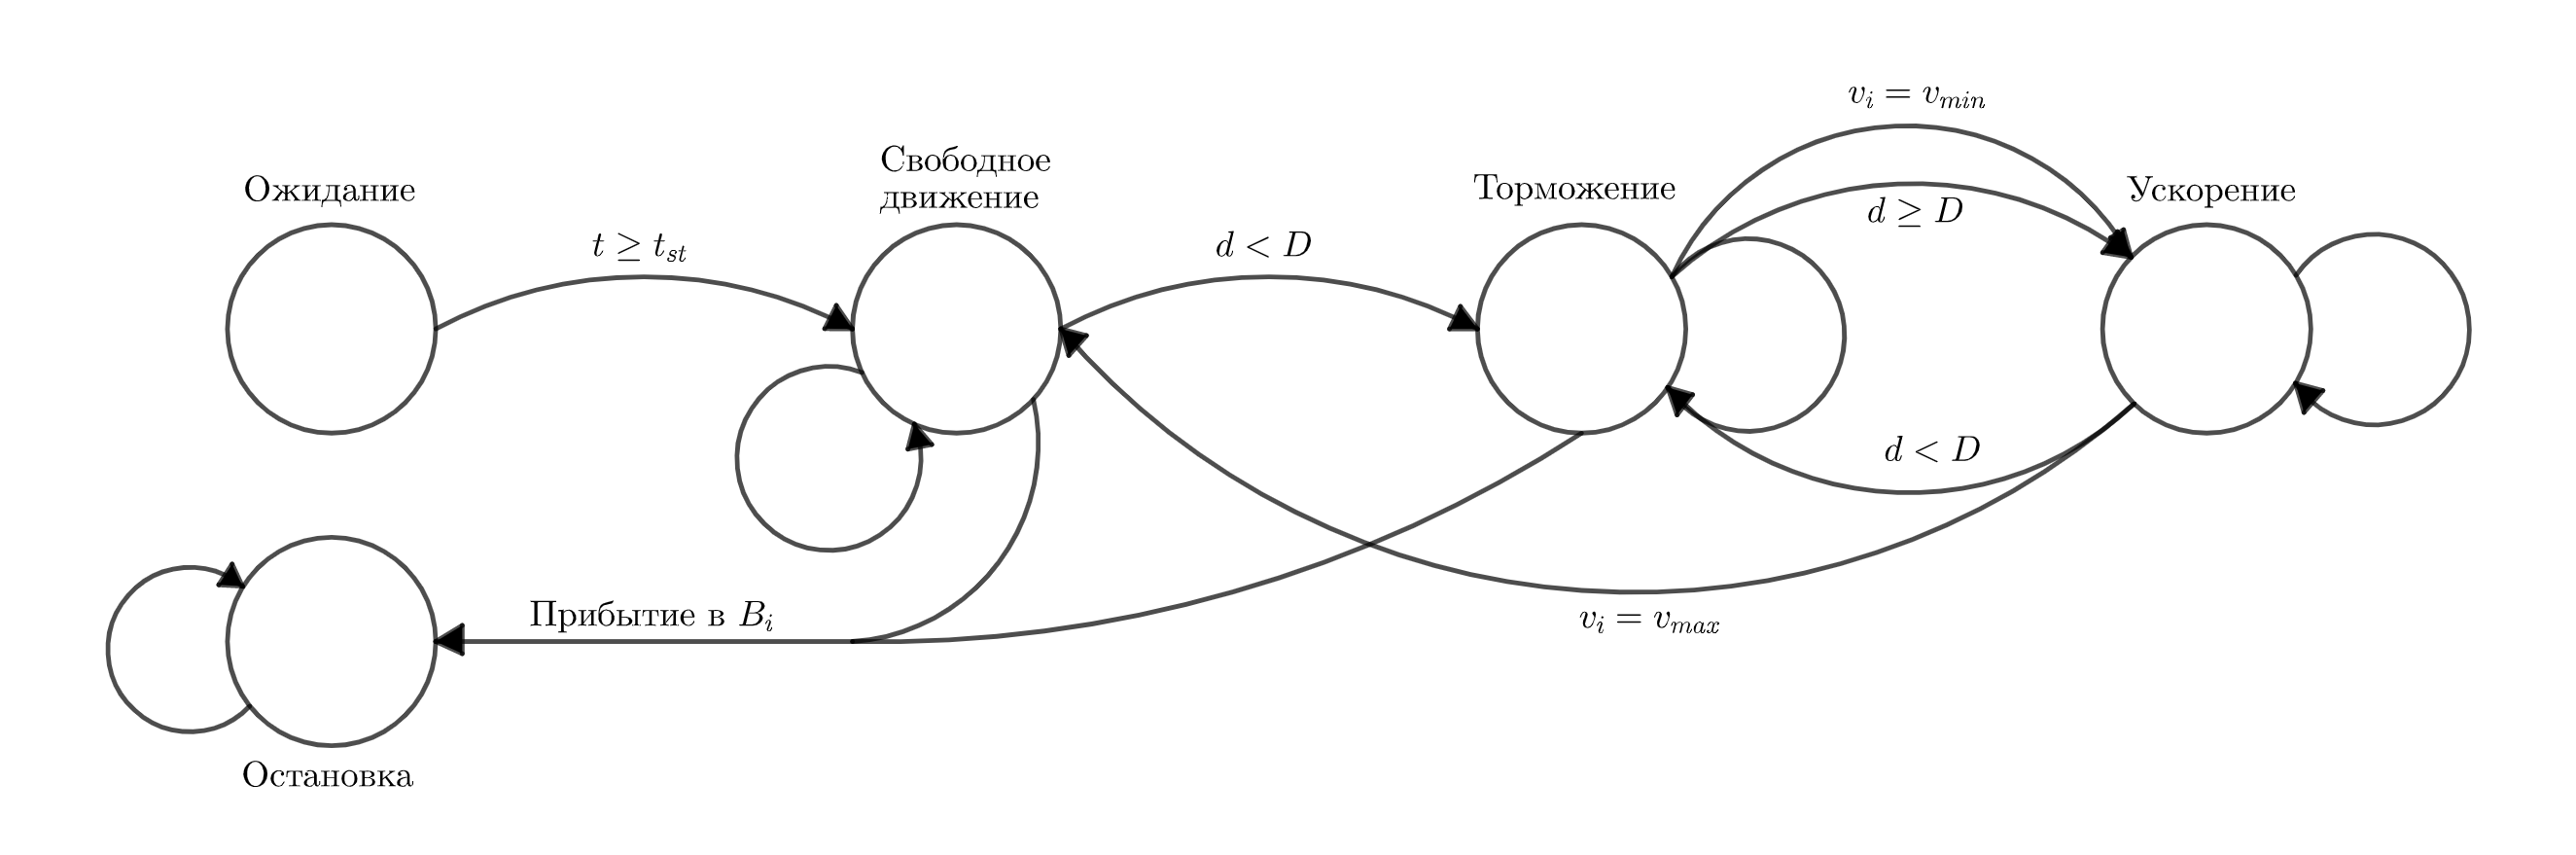
\includegraphics[scale=0.25]{example-gen.png}
		\caption{Диаграмма для $i$-ого участника в модели движения с множеством состояний $S = \{(e, x, v, t): e \in E, x \in [0, 1], v \in [v_{min}, v_{max}], t \in \mathbb{R}\}$, где $d$~-- расстояние до впереди идущего участника, $D$~-- максимальное расстояние взаимодействия с впереди идущим участником, $v_{max}$~--максимально возможная скорость, $v_{min}$~--минимально возможная скорость, $t_{st}$~-- время старта.}
		\label{ris:example_diag}
	\end{figure}
	
	Заметим, что в данном примере все зависимости с характеристикой состояния <<время в пути>> можно перенести в функции $t_i$ и $\varphi_i$. Поэтому можно рассматривать множество состояний $S = \{(e, x, v): e \in E, x \in [0, 1], v \in [v_{min}, v_{max}]\}$.
	
	Далее ограничимся только теми моделями движения, в которых все участники достигают своих заключительных состояний за конечное время. Такие модели назовем \textit{вычислимыми}.
	
	Перейдем от формального определения модели движения непосредственно к постановке задачи.
	Пусть имеется $n$ участников, которые движутся по заранее заданным маршрутам:  $ p_i = \langle E^i_{j_1}, E^i_{j_2}, \dots, E^i_{j_{m_i}} \rangle$, $ E^i_{j_k} \in E \quad i = 1, \dots, n$. Добавим к ним $(n+1)$-ого участника, которому нужно добраться из пункта $A \in V$ в пункт $B \in V$. Определим $P(A,B)$~-- множество всех простых путей из $A$ в $B$. Пусть $(n+1)$-ый участник двигается по некоторому пути $p \in P(A, B)$.
	Далее будем считать, что начальные состояния в модели движения $M$ соответствуют началам путей $p_1, \dots, p_n, p$, а заключительные --- концам этих путей. Вычислимая модель движения позволяет определить момент времени, когда $(n+1)$-ый участник достиг заключительного состояния, двигаясь по маршруту $p$. Обозначим его $T(p)$.
	
	\if 0
	Модель движения позволяет определить \textit{часть пройденного пути} для каждого АТС в зависимости от движения других участников, т.е. определить непрерывные монотонные функции
	\begin{center}
		$x_i(G, p_1, \dots, p_n, p, \cdot ) : \mathbb {R} \rightarrow [0 , 1] $, $i = 1, \dots, n+1$, $p \in P(A, B) $.
	\end{center}
	Ввиду однозначной определенности последовательности ребер $p_j$ и графа дорожной сети $G$, явную зависимость $x_i$ от данных параметров можно не указывать. 
	
	На множестве путей $P(A,B)$ определим $T(p) = \displaystyle \inf_t \{t : x_{n+1}(p, t) = 1\}$~-- время прибытия $(n+1)$-ого участника в вершину $B$ при движении по маршруту $p$. 
	\fi
	
	Требуется найти такой путь $p^* \in P(A, B)$, что $T(p^*)$ --- минимален. Другими словами, для заданной модели движения $M$ на графе дорожной сети $G(V, E, l)$ при движении $n$ участников по путям $p_1, \dots, p_n$ требуется найти такой путь $p^*$ из $A$ в $B$, что движение нового участника по этому пути $p^*$ будет \textit{оптимально}, то есть
	$$p^* = \argmin_{p \in P(A, B)} T(p).$$
	
	
	Предполагаем ничтожно малое влияние $n+1$-ого участника на движение остальных, 
	хотя такое предположение и заведомо неверно для крупногабаритных транспортных средств, для легковых автомобилей оно представляется достаточно разумным, исключая случаи аварийных ситуаций или неопытных водителей за рулем.
	
	\newpage
	\section{Модели движения}
	
	В первую очередь для решения задачи, нужно конкретизировать модели движения. Рассмотрим те из них, в которых изменения скорости участников базируются только на количестве участников на ребре в момент времени $t$. Такие модели называются \textit{макроскопическими}, а все остальные --- \textit{микроскопическими}. В этом разделе будет показано, что как макроскопические, так и микроскопические модели могут быть выражены в терминах нашей автоматной модели движения.
	
	\if 0
	%Нас интересует точное решение, поэтому промоделируем движение $n$ участников, чтобы в каждый момент времени были известны функции $x_i(t)$. 
	Поведение движения АТС в нашей постановке задачи определяется некоторой системой правил. Представим примеры таких приавил, которые описывают естественный, близкий к реальности характер движения автомобилей.
	
	Говоря о поведении движения автомобилей, мы имеем в виду изменение их скоростей в зависимости от ситуации на дороге. Для каждого АТС введем функцию \textit{скорости} \\ ${v_i(t) : \mathbb {R}_+ \rightarrow \mathbb {R}_+}$.  Обозначим через $v_m \in \mathbb {R}$ максимально возможную скорость, или \textit{скорость свободного движения}: $v_i(t) \leq v_m, \forall t \in \mathbb {R}, i = 1, \dots, n+1$.
	\fi
	
	
	\subsection{Макроскопические модели}
	
	
	%При движении $n$ участников макроскопические модели можно параметризовать набором действительных чисел $v_1, \dots, v_n$, где $v_k$~-- скорость при $k$ участниках на ребре.
	Множество состояний в макроскопических моделях движения определяется только положением на графе, т.е. $S = E \times [0, 1]$. Эти состояния
	можно разбить на $n$ классов по количеству участников на ребре (см. рис. \ref{ris:macro_diag}).  Общее количество всех возможных переходов между классами состояний для $i$~--ого участника составит $n(n-1) + 2n$.
	
	\begin{figure}[H]
		\centering
		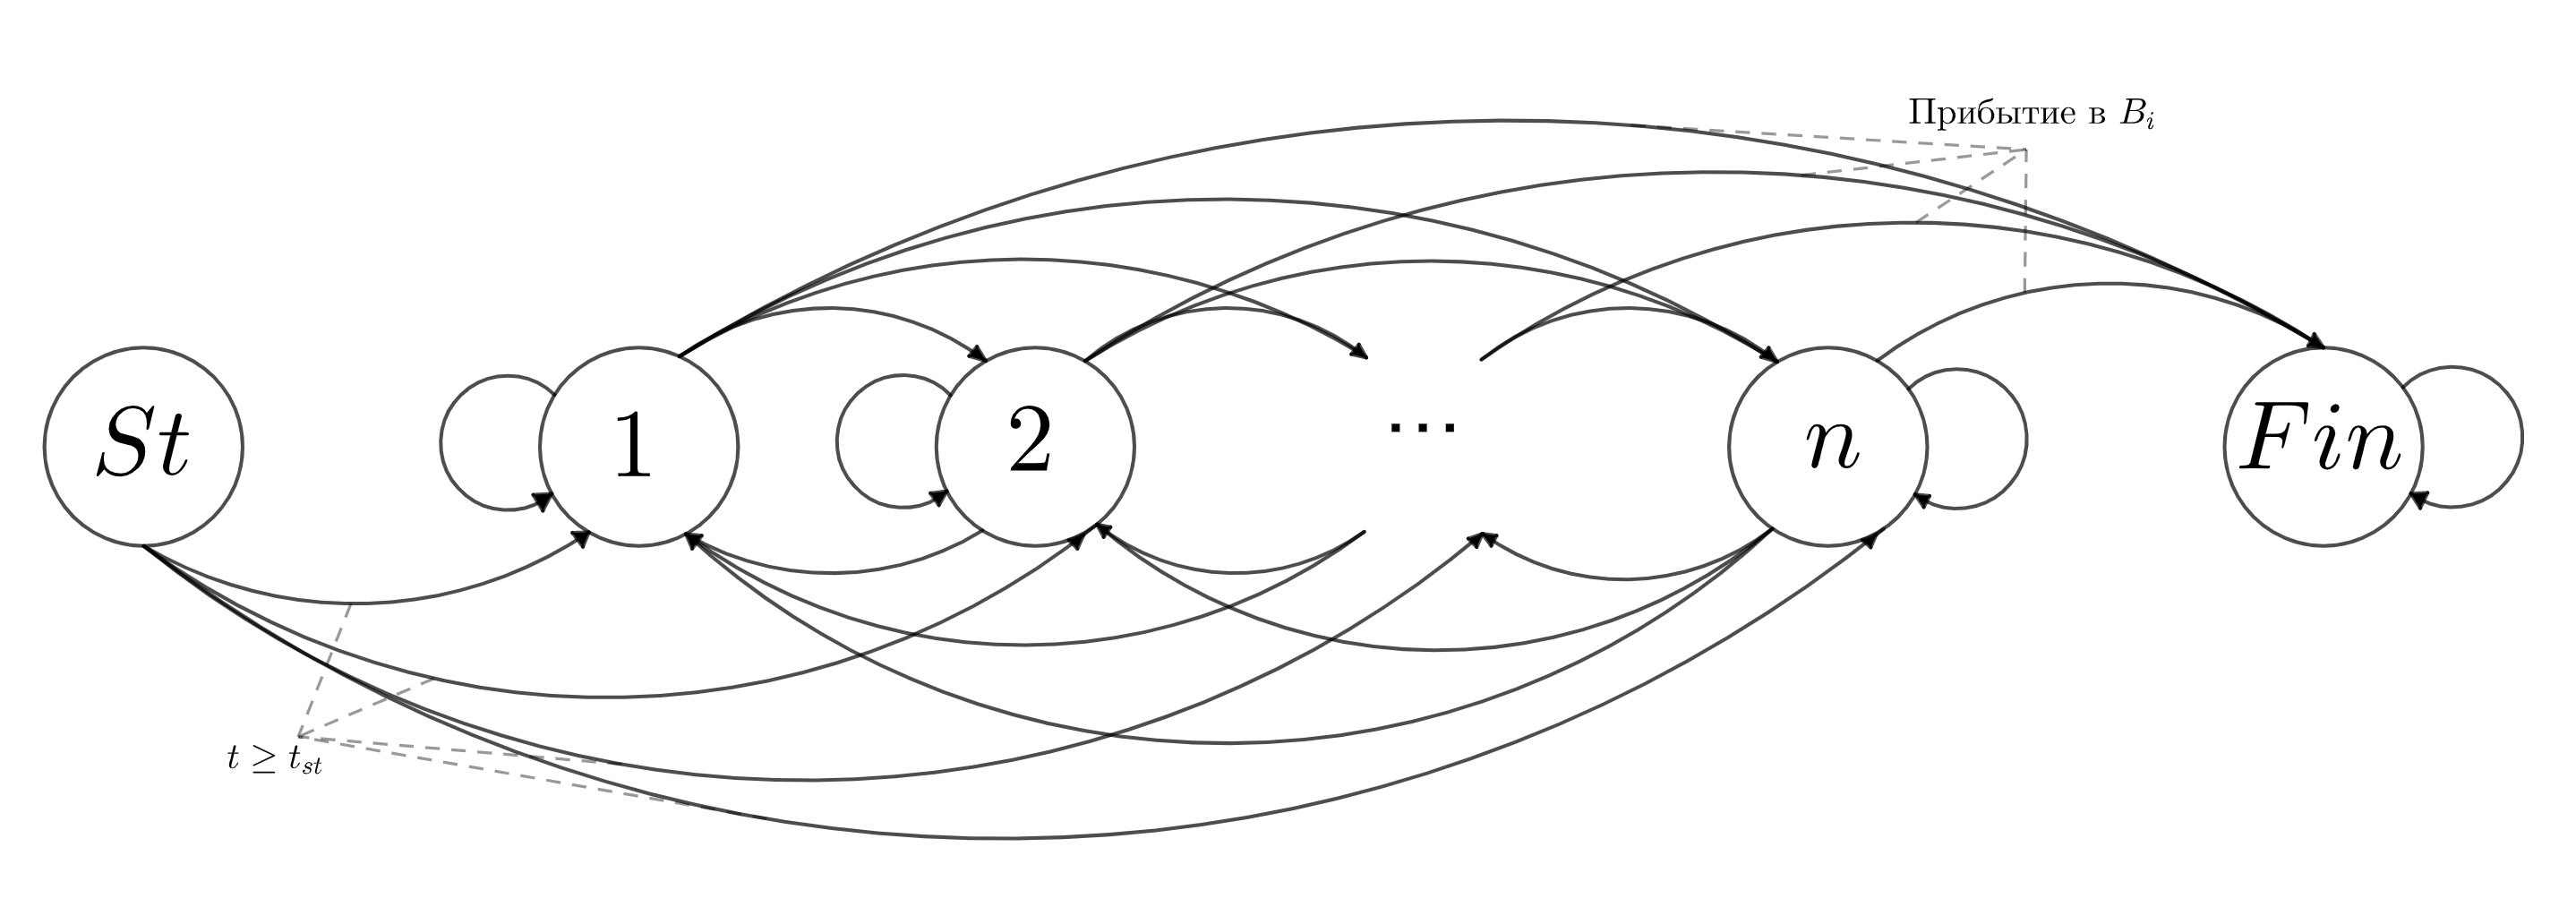
\includegraphics[scale=0.2]{Macro-gen.png}
		\caption{Диаграмма для $i$-ого участника в макроскопических моделях движения}
		\label{ris:macro_diag}
	\end{figure}
	Пусть $s_i = (e_i, x_i)$ --- положение участника $i$ на графе дорожной сети. Пусть $n_i(s_1, \dots, s_n)$ --- количество участников на ребре $e_i$. Переход из класса состояний $k$ в класс состояний $m$ осуществляется при выполнении сразу двух условий: $n_i \neq k$ и $n_i = m$. При этом критический момент для $i$~--ого участника наступает, когда какой-либо участник въезжает на ребро $e_i$ или съезжает с него:
	$$t_i = min \left\{\frac{l(e_j)\left(1-x_j\right)}{v_{n_j}} \; \bigg| \; j = 1, \dots, n; \; e_j = e_i \text{ или следующее за } e_j \text{ ребро в } p_j \text{ это } e_i\right\}.$$
	
	Для того, чтобы критические моменты $t_i, \: i = 1, \dots, n$ были определены, макроскопические модели требуют положительности скоростей $v_i, \: i = 1, \dots, n$. Условие $v_i \ge v_{min} > 0, \: i = 1, \dots, n$ обеспечивает достижимость переходов в другие классы состояний:
	$$t_i < T_i = \frac{max\{l(e_i) \: | \: e_i \in p_i\}}{v_{min}}.$$
	Количество таких переходов для участника $i$ будет ограничено количеством ребер $|p_i|$ в пути $p_i$, из чего можно сделать вывод, что все заключительные состояния достижимы, а следовательно, модель движения вычислима.
	
	Примером такой модели может послужить набор 
	\begin{equation}
		\label{eq:example_macro}
		v_k = (v_{max} - v_{min}) \left(1 - \frac{k}{n}\right)\ + v_{min}, \text{ } k \in \{1, \dots, n\}, 
	\end{equation}
	где $v_{max}, v_{min}$~-- заданные максимальная и минимальная скорости. 
	
	\subsection{Микроскопические модели}
	
	Микроскопические модели, в отличие от макроскопических, предполагают другой набор другие зависимости скоростей.
	Опишем модель \textit{следования за лидером}~-- модель, в которой поведение движения участника зависит от расстояния до впереди идущего АТС. 
	
	Пусть заданы максимальная $v_{max} > 0$ и минимальная $0 < c \le v_{min} < v_{max}$ скорости участников ($c = const$), и ускорение $a = const, \: a > 0$, которое позволяет разгоняться от $v_{min}$ до $v_{max}$. Будем считать, что участники подчиняются следующему правилу:
	% должны соблюдать \textit{безопасное расстояние} $l$~---
	оказавшись на расстоянии $d \leq l, \: l > 0$, которое мы будем называть \textit{дистанцией торможения}, до лидера, участник
	%не может к нему приближаться. В этом случае участник
	мгновенно сбрасывает свою скорость до минимальной и продолжает движение с постоянной скоростью, пока не отдалится от лидера на \textit{безопасное расстояние} $D > l$. Оказавшись на расстоянии $D$ до лидера, участник с минимальной скоростью может перейти к равноускоренному движению. Диаграмма такой модели движения представлена на рис. \ref{ris:micro_diag}.
	% Расстояние $l$ будем называть \textit{дистанцией приближения}. 
	
	\if 0
	Введем понятие \textit{дистанции видимости} или \textit{зона видимости} $D$~--- расстояние, на котором участник начинает взаимодействовать с впереди идущим лидером и в связи с этим менять свой характер движения. Также будем считать, что участники должны соблюдать \textit{безопасное расстояние} $l < D$~--- оказавшись на расстоянии $d \leq l$ до лидера, участник не может к нему приближаться. Увеличивать дистанцию между участниками позволит ускорение, которое мы зададим некоторой положительной константой.
	
	
	Пусть $i$~-ый и $(i+1)$~-ый участники, лидер и следующий за ним соотвественно, оказались в момент времени $t$ на расстоянии $d$ относительно друг друга со скоростями $v_i$ и $v_{i+1}$. Опишем характер их движения.
	
	
	\begin{enumerate}
		\item $d \ge D $
		\begin{enumerate}
			\item $v_{i+1} = v_{max} \Rightarrow a_{i+1} = 0$, продолжаем ехать с максимальной скоростью.
			\item $v_{i+1} < v_{max} \Rightarrow a_{i+1} = a_+$ на время $t = \frac{v_{max}-v_{i+1}}{a_+}$, после чего $v_{i+1} = v_{max}, a_{i+1} = 0$
		\end{enumerate}	
		\item $d \leq l \Rightarrow v_{i+1} = 0$
		\item $l < d < D $
		\begin{enumerate}
			\item $v_{i+1} \leq v_i$
			\begin{enumerate}
				\item $a_i = 0$, т.е. его движение равномерно, это может быть только в 2-х случаях:
				\begin{enumerate}
					\item $v_i = v_{max} \Rightarrow a_{i+1} = a_+$ на время $t = \frac{v_{max}-v_{i+1}}{a_+}$, после чего $v_{i+1} = v_{max}, a_{i+1} = 0$
					\item $v_i = 0$, едем время $t = \frac{d-l}{v_{i+1}}$, не меняя скорость, после чего останавливаемся, $v_{i+1} = 0$.
				\end{enumerate}	
				\item $a_i \neq 0 \Rightarrow a_{i+1} = a_i$ 
			\end{enumerate}
			\item $v_{i+1} > v_i$ 
			\begin{enumerate}
				\item $a_i = a_+ \Rightarrow a_{i+1} = a_-$ до момента, когда $v_i + a_it = v_{i+1} + a_{i+1}t$ или $v_{i+1}$ станет $0$, т.е. до $t = min\left(\frac{2Dl(v_{i+1}-vi)}{v^2_{max}(l+D)}, \frac{2lv_{i+1}}{v^2_{max}}\right)$,  после чего $a_{i+1} = a_i = a_+$. 
				\item $a_i = a_- \Rightarrow a_{i+1} = a_i = a_-$.
			\end{enumerate}	
		\end{enumerate}
	\end{enumerate}
	
	\fi
	\begin{figure}[H]
		\centering
		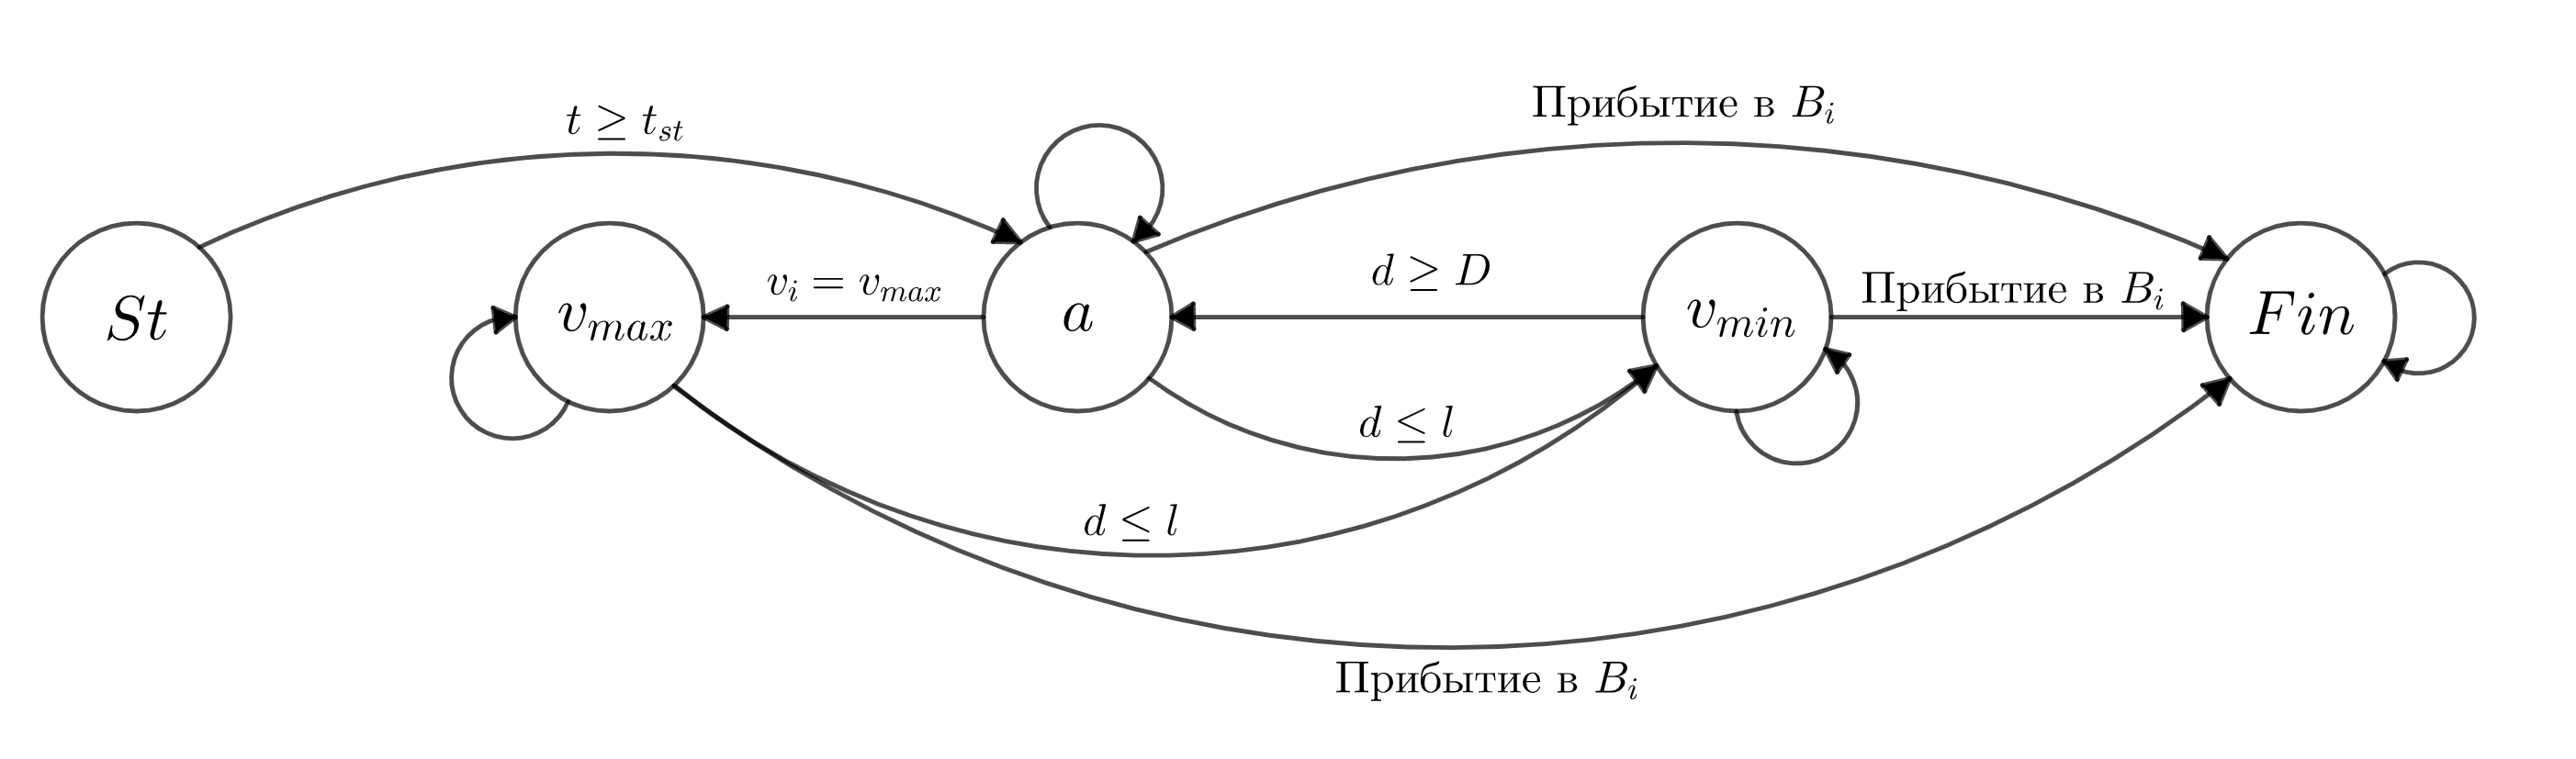
\includegraphics[scale=0.2]{Micro-gen.png}
		\caption{Диаграмма для $i$-ого участника в модели следования за лидером.}
		\label{ris:micro_diag}
	\end{figure}
	
	В данной модели множество состояний есть $S = \{(e, x, v): e \in E, x \in [0, 1], v \in [v_{min}, v_{max}]\}$.
	
	Для каждого перехода между классами состояний время ограничено снизу положительной константой, т.к. разгон до максимальной скорости и отдаление от лидера происходят не мгновенно. Поскольку минимальная скорость также ограничена снизу, каждый участник достигнет конца своего пути. Следовательно, описанная модель движения является вычислимой.
	
	\newpage
	\section{Моделирование}
	
	%Под моделированием будем понимать воспроизведение движения всех АТС по установленным правилам.
	Под моделированием будем понимать воспроизведение движения $n+1$ участника, движущихся по путям $p_1, \dots, p_n, p, \; p \in P(A, B)$ в модели движения $M = M(p_1, \dots, p_n, p)$.
	Рассмотрим алгоритм нахождения времени, затраченного $n+1$-ым участником на путь $p$.
	
	\begin{algorithm}[H]
		\caption{Моделирование движения участников}
		\label{alg:modeling}
		{\bf {Input:}} количество участников $n+1$, граф дорожной сети $G$, модель движения $M = M(p_1, \dots, p_n, p)$, набор начальных состояний $s^{\circ}_1, \dots, s^{\circ}_{n+1}$\\
		{\bf {Output:}} $T(p)$\\
		{\bf {Data:}} текущее время $t$, критический момент движения $i$-ого участника $t^*_i$, критический момент $t^*$
		\begin{algorithmic}[1]
			\State $t = 0$
			\For{$i = 1, \ldots, n+1$}
			\State $s_i \gets s^{\circ}_i$
			\EndFor
			\While{$ s_{n+1} \notin F$}
			\For{$i = 1, \ldots, n+1$}
			\State $t^*_i \gets t_i(s_1, \dots, s_{n+1})$ 
			\EndFor
			\State $t^* \gets min \left(t^*_1, \dots, t^*_{n+1} \right)$
			\For{$i = 1, \ldots, n+1$}
			\State $s_i \gets \varphi_i(s_1, \dots, s_{n+1}, t^*)$
			\EndFor
			\State $t \gets t^*$
			\EndWhile
			\State $T(p) \gets t$
		\end{algorithmic}
	\end{algorithm}

	Процесс моделирования представляет собой последовательную смену состояний участников. Поэтому для сложности алгоритма $S_M (p_1, \ldots, p_n, p)$ верно 
	$$S_M (p_1, \ldots, p_n, p) = S_{\phi, t} (p_1, \ldots, p_n, p) N_{t} (p_1, \ldots, p_n, p),$$ где $S_{\phi, t},$ --- сложность обновления на шаге 6 - 13, а $N_{t}$ --- количество смен состояний, то есть количество циклов шага 5.
	
	Опишем сложность моделирования макроскопической модели. Количество смен состояний в такой модели равно количеству смен ребер. Поэтому $N_{t} (p_1, \ldots, p_n, p) = |p| + \sum\limits_{i = 1}^n|p_i|$. Количество операций при обновлении состояний зависит от $n$ линейно. Таким образом, сложность моделирования составляет $S_M (p_1, \ldots, p_n, p)= n \left(|p| + \sum\limits_{i = 1}^n|p_i|\right)$.
	
	\if 0
	
	Рассмотрим 2 различных способа моделирования с $(n+1)$-ым участником: 
	\begin{enumerate}
		\item он влияет на движение $n$ участников и вследствие на самого себя;
		\item движение $n$ участников не зависит от добавленного АТС.
	\end{enumerate}
	
	\subsection{Независимость движения участников от добавленного АТС}
	\subsection{Взаимосвязь движений нового участника и группы АТС}
	
	\fi
	\newpage
	\section{Поиск оптимального пути}
	
	Отметим, что количество путей конечно, поэтому первое, что приходит на ум в качестве решения, это перебор всех возможных путей и нахождение подходящего по затраченному времени. Посчитаем сложность этого алгоритма и сделаем вывод о его использовании в нашей задаче на практике.
	
	\subsection{Перебор. Сложность}
	Чтобы узнать, применим ли перебор в нашем случае, посчитаем сложность нахождения кратчайшего пути среди множества всех простых путей из $A$ в $B$. Пусть $S_M(p_1, \ldots, p_n, p)$~-- сложность моделирования, т.е. нахождения времени $T(p)$, потраченного на путь $p$.
	%функции $x^p_{n+1}(t)$, при выборе пути $p$.
	Тогда сложность перебора
	\begin{center}
		$S = \sum\limits_{p \in P(A,B)} S_M(p_1, \ldots, p_n, p) = \vert P(A,B) \vert \overline S_M$, где $\overline S_M$~-- средняя сложность моделирования.
	\end{center}
	Заметим, что $ S $ растет при увеличении количества возможных путей. Так, в полном графе на $\vert V \vert$ вершинах получим $S = \left(\sum\limits_{k = 1}^{|V| - 2} k!\right)^n \overline S_M$.
	
	В качестве примера можем рассмотерть также регулярный граф-решетку на $\mathbb {R}^2$ и на нем оценить снизу сложность поиска пути с минимальными тратами. Пусть точки $A$ и $B$ имеют координаты $(a_1, a_2)$ и $(b_1, b_2)$ соответственно. Тогда количество путей минимальной длины в метрике Манхэтенна будет составлять $C^{|a_1-b_1|}_{|a_1-b_1| + |a_2-b_2|}$. Понятно, что путей $|P(A,B)|$ в таком графе гораздо больше. Таким образом, получаем оценку снизу для регулярного решеточного графа
	
	\begin{center}
		$C^{|a_1-b_1|}_{|a_1-b_1| + |a_2-b_2|} \overline S_M  \leq  \vert P(A,B) \vert \overline S_M = S$.
	\end{center}
	
	Например, в решетке-квадрате со стороной $m$ при движении из угловой точки по диагонали в угловую точку напротив количество путей минимальной длины составит $C^m_{2m} = \frac{(2m)!}{m!m!} $. По формуле Стирлинга
	\begin{center}
		$ C^m_{2m} = \frac{\sqrt{2\pi(2m)} \left( \frac{2m}{e} \right)^{2m} + \tilde{o}(1)}{\left(\sqrt{2\pi m} \left( \frac{m}{e} \right)^m + \tilde{o}(1)\right)  \left(\sqrt{2\pi m} \left( \frac{m}{e} \right)^m + \tilde{o}(1)\right)} = \frac{2\sqrt{\pi m} \left( \frac{2m}{e} \right)^{2m}}{2\pi m \left( \frac{m}{e} \right)^{2m}} + \tilde{o}(1) = \frac{2^{2m}}{\sqrt{\pi m}} + \tilde{o}(1)$.
	\end{center}
	Понятно, что при увеличении $m$, количество путей экспоненциально растет.
	
	С помощью перебора можно находить кратчайшие пути быстро, если $|P(A,B)|$ не велико. Однако изначально наша задача была сформулирована в терминах дорожной сети и предполагала графы с достаточно большим количеством вершин и ребер, что влияет на количество маршрутов для заданных точек. Таким образом, можно сделать вывод, что в общем случае перебор путей в нашей задаче на практике не применим.
	
	\newpage
	\subsection{Поиск кратчайшего пути в динамическом графе}
	
	Граф $G(V, E)$ будем называть  \textit{динамическим}, если на его ребрах определены динамические затраты $\phi_e(t) : \mathbb {R}_+ \rightarrow \mathbb {R}, \; e \in E$. Если мы оказались в начальной вершине ребра $e$ в момент времени $t$, то время преодоления ребра будет равняться $\phi_e(t)$.
	
	Рассмотрим путь $p = \langle V_0, e_1, V_1, e_2, V_2, \dots, V_{k-1}, e_k, V_k \rangle $, начало движения происходит в вершине $V_0$ в момент времени $t_0$, а вершину $V_i$ мы посещаем в некоторый момент времени $t_i$. Тогда 
	\begin{align*}
		%t_0 & = t,  \\
		t_1 & = \phi_{e_1}(t) + t = \phi_{e_1}(t_0) + t_0,  \\
		t_2 & = \phi_{e_2}(\phi_{e_1}(t) + t) + \phi_{e_1}(t) + t = \phi_{e_2}(t_1) + t_1, \\
		& \dots \\
		t_i & = \phi_{e_i}(t_{i-1}) + t_{i-1}, \\
		& \dots \\
		t_k & = \phi_{e_k}(t_{k-1}) + t_{k-1}.
	\end{align*}
	Пусть $P(A, B)$~-- множество всех простых путей из $A$ в $B$ в динамическом графе $G(V, E)$. Необходимо найти путь из $A$ в $B$, который требует минимальных затрат, т.е. 
	\begin{equation}
		\label{add_task}
		\widehat{p} = \argmin_{p \in P(A, B)} t_{|p|}.
	\end{equation}
	Множество всех решений задачи \eqref{add_task} обозначим $\widehat{P}(A, B)$.
	
	В общем случае функции временных затрат могут быть любыми. Давайте рассмотрим эту задачу с дополнительным условием на $\phi_e(t)$:
	
	\begin{equation}
		\label{eq:neravenstvo_prohojdenya}
		\phi_e(t) <\Delta t + \phi_e(t + \Delta t), \quad \Delta t > 0
	\end{equation}
	Назовем условие \eqref{eq:neravenstvo_prohojdenya} \textit{неравенством прохождения ребер}. Утверждается, что если для $\forall e \in E$ функции временных затрат $\phi_e$ удовлетворяют неравенству прохождения ребер, то задачу можно решить модифицированным алгоритмом Дейкстры.
	
		\begin{lemma}
		\label{lemma:uslovie}
		Пусть для функции $\phi_e(t)$ выполняется условие \eqref{eq:neravenstvo_prohojdenya}. Множество решений задачи \eqref{add_task} есть $\widehat{P} (A, B) \subset P (A, B)$. Рассмотрим вершину $C$ - вершина из некоторого пути $\widehat{p} \in \widehat{P} (A, B)$. Ограничим  путь $\widehat{p}$ вершиной $C$ и обозначим такой путь как  $\pi_C(\widehat{p})$. Тогда верно $\pi_C(\widehat{p}) \in \widehat{P} (A, C)$.  
	\end{lemma}
	
	\begin{proof}
		От противного. Предположим $\pi_C(\widehat{p}) \notin \widehat{P} (A, B)$. Без ограничения общности считаем, что в $G$ нет кратных ребер, и $C$ --- предпоследняя точка пути $p$. Тогда можно считать, что $\widehat{p} = p_1DCB$, где $p_1$ --- некоторый некоторый путь из $A$. Значит, $\pi_C(\widehat{p}) = p_1DC$. 
		
		
		Рассмотрим некоторый $\widehat{q} = p_2FC \in \widehat{P} (A, C)$. Тогда верно
		\begin{equation}
			\label{eq:nervo}
			t_F^{p_2} + \phi_{FC}(t_F^{p_2}) < t_D^{p_1} + \phi_{DC}(t_D^{p_1}),
		\end{equation}
		где $t_F^{p_2}$ --- время прибытия в вершину $F$ через путь $p_2$, $t_D^{p_1}$ --- время прибытия в  вершину $D$ через путь $p_1$. Обозначим за $t_{C}^{p_2F}$ и $t_{C}^{p_1D}$ левую и правую часть неравенства \eqref{eq:nervo} соответственно. В новых обозначениях $t_{C}^{p_2F} < t_{C}^{p_1D}$.
		Рассмотрим путь $q = \widehat{q}B =  p_2FCB \in P (A, B)$. Поскольку $\widehat{p}$ - решение задачи имеем 
		\begin{equation*}
			\label{eq:nervo_reshenie1}
			t_{C}^{p_2F} + \phi_{CB}(t_{C}^{p_2F}) \ge t_{C}^{p_1D} + \phi_{CB}(t_{C}^{p_1D}).
		\end{equation*}
		или, 
		\begin{equation}
			\label{eq:nervo_reshenie2}
			\phi_{CB}\left(t_{C}^{p_2F}\right) \ge \left(t_{C}^{p_1D} - t_{C}^{p_2F}\right) + \phi_{CB}\left(t_{C}^{p_2F} + \left(t_{C}^{p_1D} - t_{C}^{p_2F}\right)\right).
		\end{equation}
		Противоречие с условием \eqref{eq:neravenstvo_prohojdenya}, где $\Delta t = t_{C}^{p_1D} - t_{C}^{p_2F} > 0$.
	\end{proof}
	
	Таким образом, лемма \ref{lemma:uslovie} утверждает, что любой подпуть оптимального пути задачи \eqref{add_task} является оптимальным, а условие \eqref{eq:neravenstvo_prohojdenya} является достаточным признаком выполнения такого свойства.
	
	\subsubsection{Модифицированный алгоритм Дейкстры}
	
	Для каждой вершины будем хранить два значения: минимальное время, за которое можно добраться до этой вершины, и ребро, через которое проходит кратчайший маршрут до вершины.
	Применяем стандартный алгоритм Дейкстры, с отличием, что при посещении вершины мы фиксируем время для нее и пересчитываем функции временных затрат на всех ребрах, исходящих из этой вершины.
	
	\begin{state}
		\label{utv:Deikstra}
		Пусть для функции $\phi_e(t)$ выполняется условие \eqref{eq:neravenstvo_prohojdenya}. Тогда алгоритм Дейкстры для каждого $B \in V$ позволяет найти хотя бы одно решение задачи \eqref{add_task}.
	\end{state}
	
	\begin{proof}
		Обозначим $t(v)$ --- минимальные затраты в задаче \eqref{add_task} с $v \in V$, $d(v)$ --- затраты на вершине $v \in V$, обновляемые в ходе работе алгоритмом. Докажем по индукции, что в момент посещения любой вершины $B$ выполняется равенство  $d(v) = t(v)$.
		
		\textit{База}. Первая посещаемая вершина есть $A$. В этот момент $d(A) = t(A) = t_0$.
		
		\textit{Шаг}. Пусть мы выбрали для посещения вершину $B \ne A$. Докажем, что в этот момент $d(B) = t(B)$. Для начала отметим, что для любой вершины $v \in V$ всегда выполняется $d(v)\ge t(v)$, поскольку алгоритм не может найти путь с затратами меньше минимальных. Пусть $\widehat{p}$ — путь из $A$ в $B$ с минимальными затратами.
		Вершина $B$ находится на $\widehat{p}$ и не посещена. Поэтому множество непосещённых вершин на $\widehat{p}$ непусто. Пусть $C$ --- первая непосещённая вершина на $\widehat{p}$, $D$ --- предшествующая ей, и ,следовательно, посещённая. Поскольку путь $\widehat{p}$ оптимальный, то по лемме \ref{lemma:uslovie} его часть, ведущая из $A$ через $D$ в $C$, тоже оптимальна, следовательно $t(C) = t(D) + \phi_{DC}(t(D))$.

		По предположению индукции, в момент посещения вершины $D$ выполнялось $d(D) = t(D)$, следовательно, вершина $C$ тогда получила затраты не больше чем $t(D) + \phi_{DC}(t(D)) = t(C)$. Следовательно, $d(C) = t(C)$. Если $C = B$, то шаг индукции доказан. Иначе, поскольку сейчас выбрана вершина $B$, а не $C$, затраты $d(B)$ минимальны среди непосещённых, то есть $d(B) \le d(Y) = t(Y) \le t(B)$. Учитывая, что $d(B) \ge t(B)$, имеем $d(B) = t(B)$, что и требовалось доказать.
		
		Поскольку алгоритм заканчивает работу, когда все вершины посещены, в этот момент $d(v) = t(v), v \in V$.
	\end{proof}
	\begin{figure}[H]
	\centering
	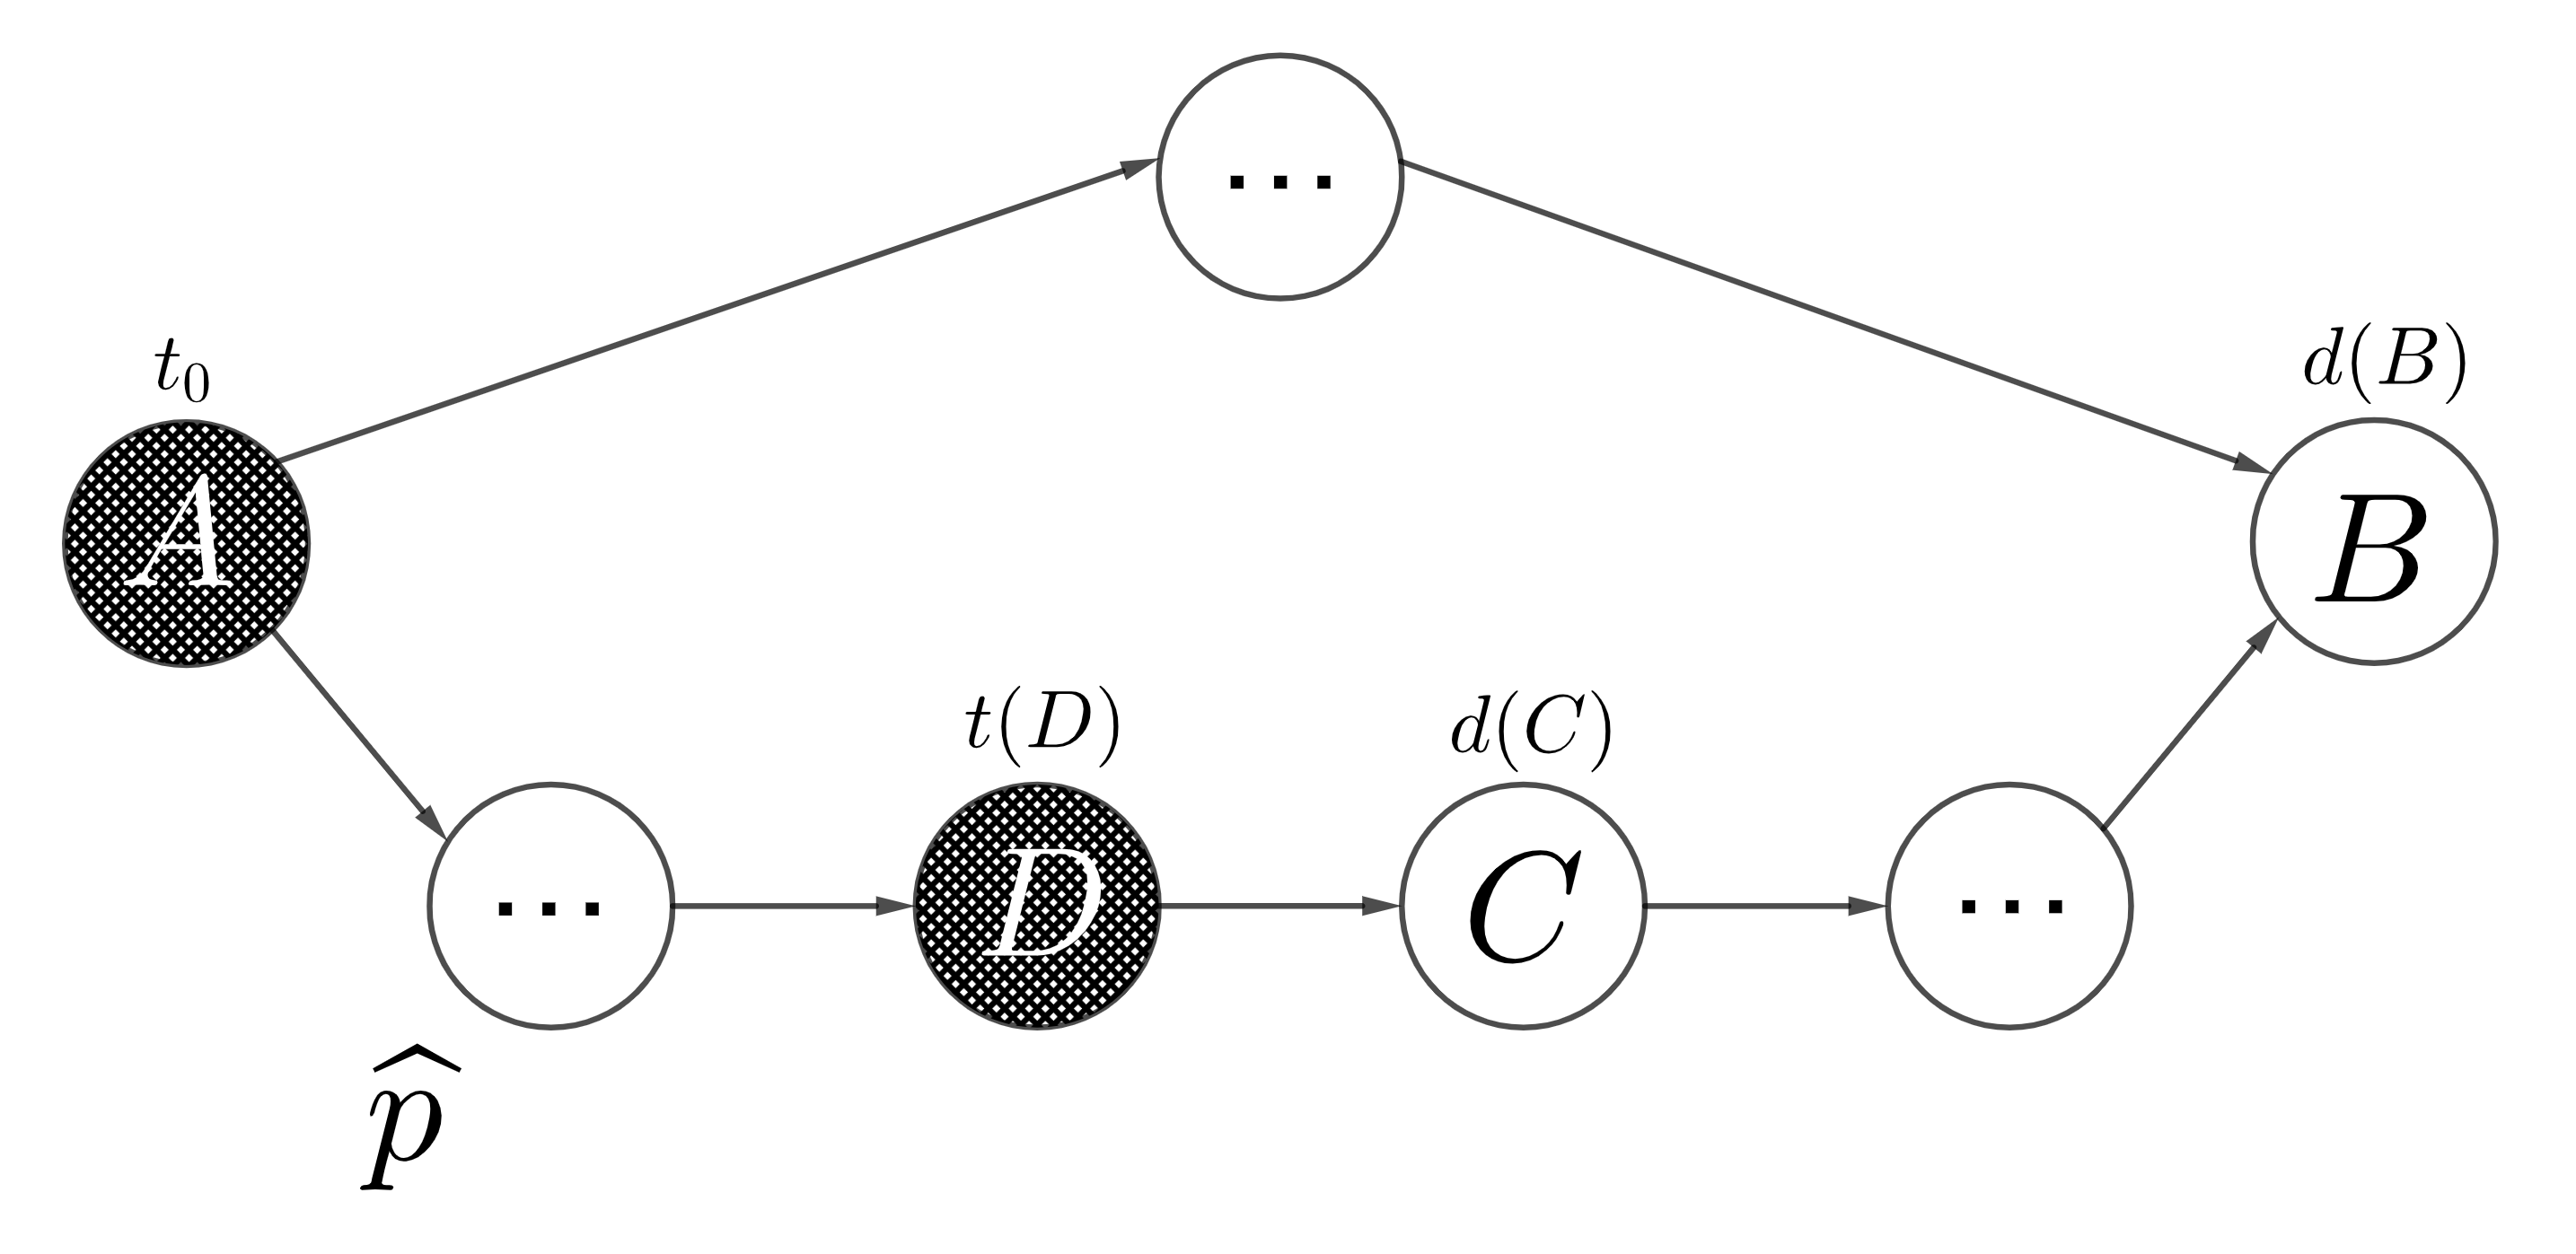
\includegraphics[scale=0.25]{Deikstra.png}
	\caption{Шаг индукции в доказательстве утверждения \ref{utv:Deikstra}.}
	\label{ris:Deikstra-graph}
	\end{figure}

	Если $\overline S_{\phi}$~-- средняя сложность вычисления функций $\phi_e, \; e \in E$, то средняя сложность модифицированного алгоритма Дейкстры есть $S = |E|\overline S_{\phi}.$\\
	
	Понятно, что если неравенство прохождения ребер не выполняется, то модифицированный алгоритм Дейкстры может построить не кратчайший маршрут в терминах временных затрат. Рассмотрим такой пример (рис. \ref{ris:deikstra}). Пусть $\phi_e(t)$~--- время, которое требуется на прохождение ребра $e$. Пусть из $A$ в $C$ ведут два ребра с временными затратами $1$ и $2$, а время, необходимое для преодоления ребра $CB$, зависит от момента начала движения по этому ребру. Другими словами, если в вершине $C$ мы оказались позже, а именно, в момент времени $t > 1.5$, то времени на участок $CB$ понадобится меньше (например, мы пропустили час-пик, и загруженность дорог стала меньше). Тогда временные затраты возможных путей в таком графе:
	\begin{align*}
		p_1: & \\
		& t_0 = 0 \\
		& \phi_{AC}(t) = 1  \\
		& \phi_{CB}(t) = 1 + 2 \mathbb{I} \{t < 1.5\} \\
		p_2: & \\
		& t_0 = 0 \\
		& \phi_{AC}(t) = 2  \\
		& \phi_{CB}(t) = 1 + 2 \mathbb{I} \{t < 1.5\} 
	\end{align*}
	Время прохождения пути $p_1$ будет составлять $t_{p_1} = t_0 + \phi_{AC}(t_0) + \phi_{CB}(\phi_{AC}(t_0)) = 1 + 3 = 4 $. Время прохождения пути $p_2$ будет составлять $t_{p_2} = 2 + 1 = 3 $. Очевидно, на путь $p_2$ потребуется меньше времени, чем на путь $p_1$, но алгоритм Дейкстры предложит в качестве решения задачи маршрут $p_1$.
	
	\begin{figure}[H]
		\centering
		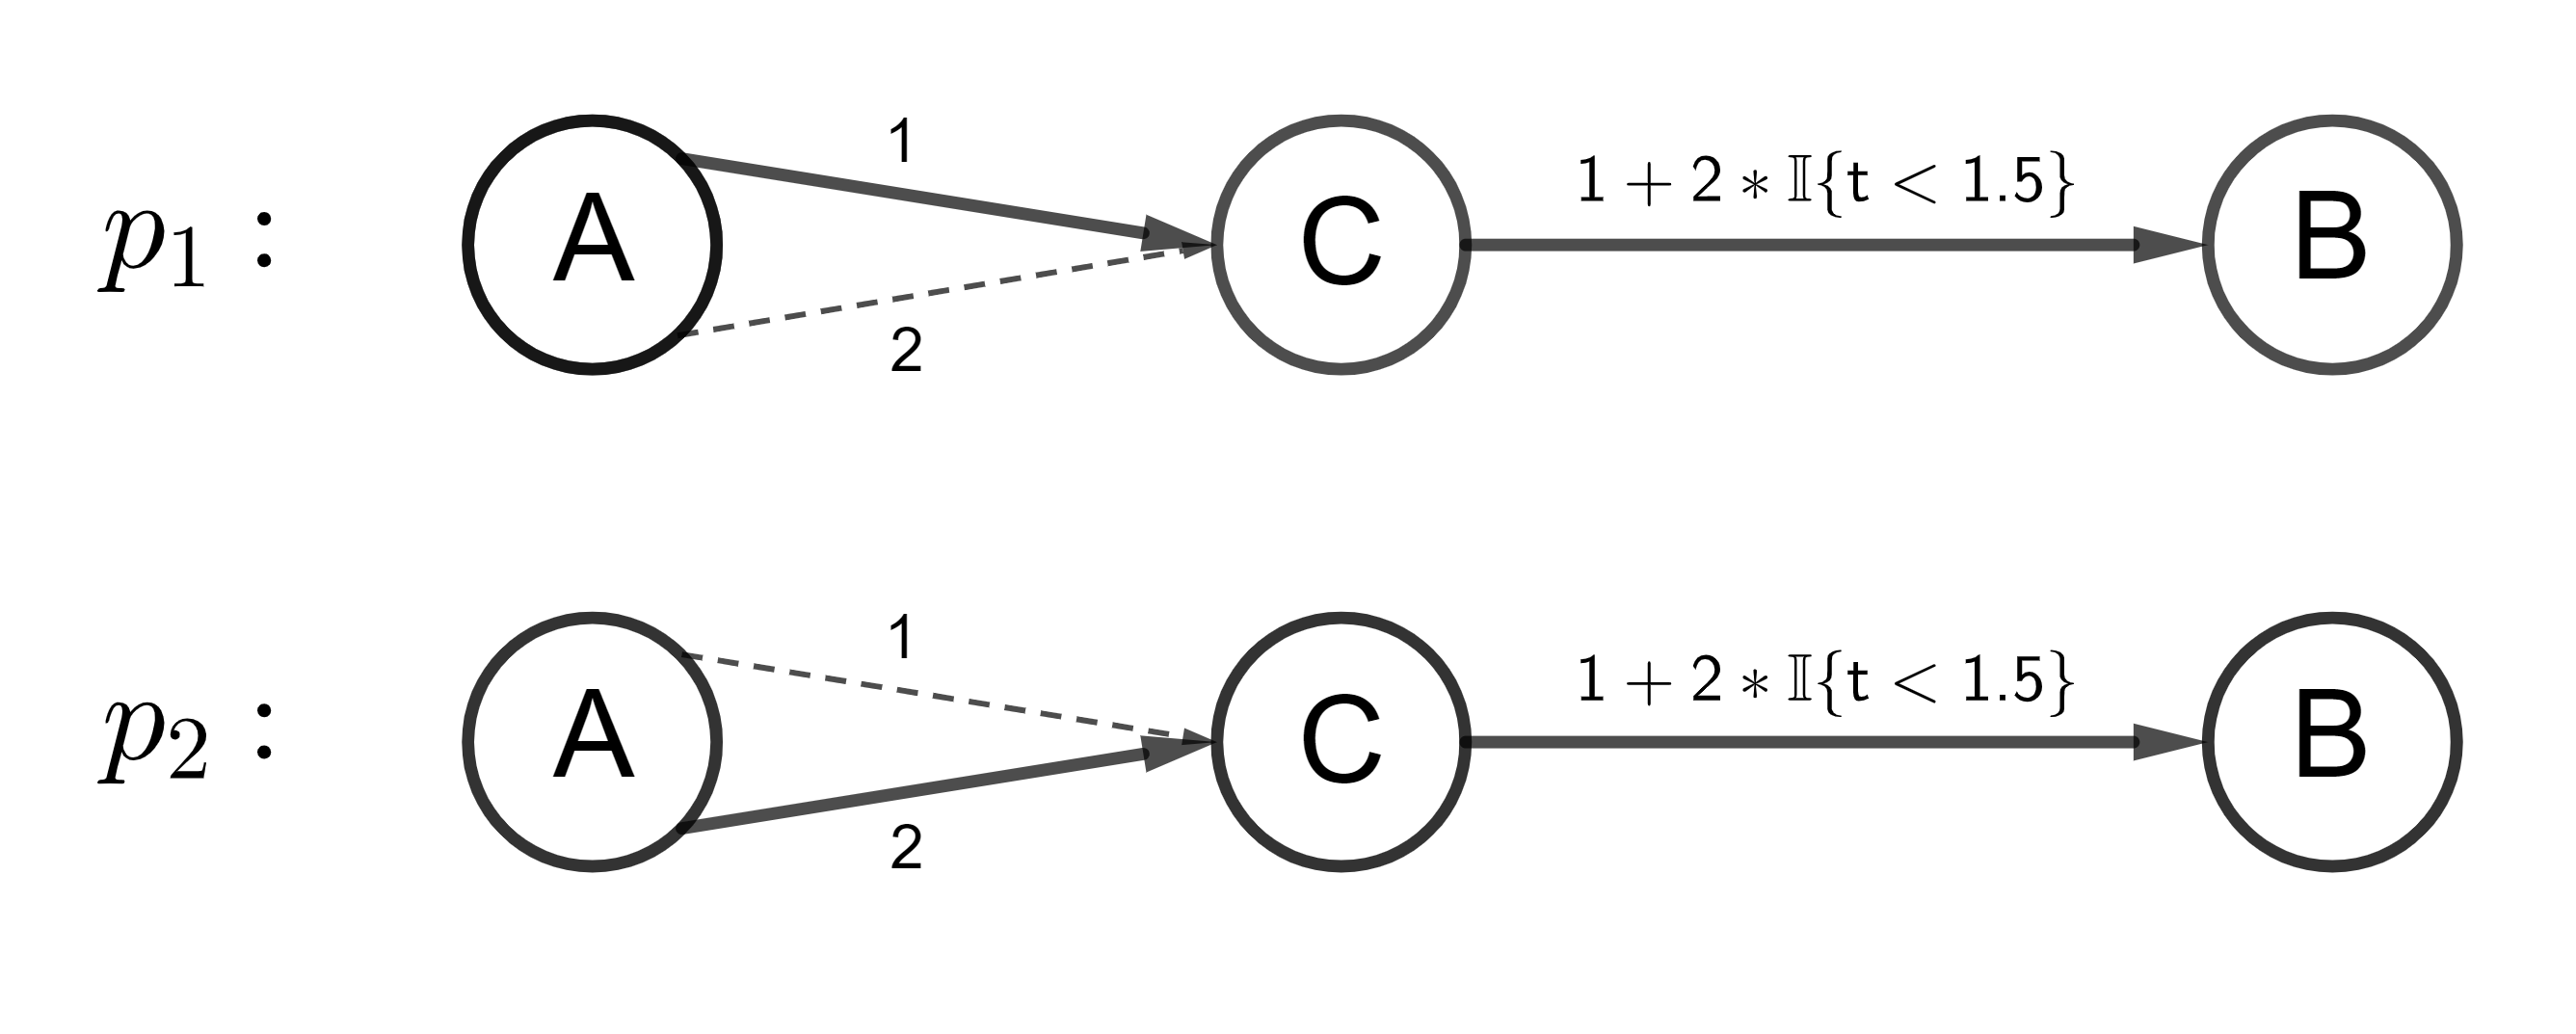
\includegraphics[scale=0.2]{graph_2.png}
		\caption{Пример графа с невыполненным условием неравенства прохождения ребер.}
		\label{ris:deikstra}
	\end{figure}
	
	Отметим, что наша задача поиска оптимального маршрута сводится к вспомогательной задаче. Правила движения участников и их взаимодействий определяют функции $\phi_e$, $e \in E $. Значения этих функций можно получить путем моделирования движения. Тогда $\overline S_{\phi} = \overline S_M$ и $S = |E|\overline S_M$.
	
	Неравенство прохождения ребер можно переформулировать так: дорожная сеть обладает условием FIFO --- если участник $i$ въехал на дорогу позже участника $j$, то $i$-ый участник покинет ее не раньше $j$-ого. Другими словами, если участники не обгоняют друг друга, то путь с минимальными затратами можно найти при помощи алгоритма Дейкстры.
	
	\subsubsection{Применимость модифицированного алгоритма Дейкстры}
	
	%Тут какое-то утверждение про то, что 	Если в модели движения $M$ процесс моделирования движения зависит только от положения участника на ребре, то в $M$ выполняется неравенство прохождения ребер.
	Поскольку неравенство прохождения ребер является гарантией того, что модифицированный алгоритм Дейкстры дает оптимальное решение, мы хотели бы исследовать выполнение этого неравенства в интересующих нас моделях движения. Оказывается, что для любой макроскопической модели верно 
	
	\begin{state}
		Пусть в модели движения $M$ известно, что выбор пути участника $n+1$ не влияет на движение других участников. Предположим, что состояния в модели движения описываются только положением участника на графе, то есть $S = E \times [0, 1]$. Тогда в $M$ выполняется неравенство прохождения ребер \eqref{eq:neravenstvo_prohojdenya} для участника $n+1$.
	\end{state}
	
	\begin{proof}
		Докажем от противного. Рассмотрим одного участника и его копию, которая могла двигаться в другое время по дургому ребру. Пусть в какой-то момент копия участника $n+1$ приехала в ребро раньше, чем другая копия, однако выехала из ребра позже. Тогда существует момент времени и состояние, для которых $s_{n+1}^1(t)  = s_{n+1}^2(t)$. Тогда $s_i^1(t) = s_i^2(t)$, $i = 1, \ldots, n + 1$. Поскольку процесс моделирования можно обратить, получим, что обе копии приехали в это ребро одновременно. Противоречие.
	\end{proof}
	
	\if 0
	
	И участник, и копия зависят от движений других участников, но друг на друга не влияют. Итак, пусть участник въезжает на ребро $e$ в разные моменты времени $t_1$ и $t_2$, $t_2 > t_1$ с ребер $e_1$ и $e_2$ соответственно. Пусть $x(t)$~-- часть пройденного ребра $e$. Предположим, что $\phi_e(t_1) > (t_2-t_1) + \phi_e(t_2)$, тогда в какой-то момент времени $t$ $x_1(t) = x_2(t) \; \Rightarrow  $ участник и его копия попадают в одно состояние $s \in S$, но так как при $M$ состояния участника зависят только от $x(t)$, то в любой момент времени состояния участника и его копии должны совпадать,
	
\end{proof}
\fi


%Потом говортся, что макроскопические все такие хорошие и супер--пупер


В микроскопических моделях условия выполнимости неравенства не найдены, а как мы уже выяснили на примере (см. рис. \ref{ris:deikstra}), модифицированный алгоритм Дейкстры может выдать не оптимальное решение задачи, если неравенство прохождения ребер не выполнено. Беря во внимание этот факт, мы предлагаем не отказываться от применения алгоритма и к микроскопическим моделям. Для них можно посчитать погрешность алгоритма.

Обратимся к описанной нами микроскопической модели (см. рис. \ref{ris:micro_diag}) и рассмотрим случай, когда участник мог бы <<обогнать>> самого себя, если бы начал движение позднее. Опишем худший случай в нашей модели на бесконечном ребре. Участник оказывается на расстоянии $d \approx 0$ до лидера и теряет свою скорость до $v_{min}$. Пусть лидер и участник со сдвигом по времени двигаются со скоростями $v_{max}$ на расстоянии $l+\varepsilon, \: \varepsilon > 0$ друг от друга и они не меняют своих скоростей. В таком случае участнику, близкому к лидеру, нужно отдалиться на безопасное расстояние $D$ за $t_1 = \frac{D}{v_{max}-v_{min}}$ и разогнаться до скорости $v_{max}$ за $t_2 = \frac{v_{max}-v_{min}}{a}$. За это время $t = t_1 + t_2$ участник со сдвигом преодолеет расстояние $s = v_{max}t$. Расстояние между участником и его копией через время $t$ составит
$$\Delta s =  D - l + \frac{\left(v_{max}-v_{min}\right)^2}{2a}.$$
Такая разница в расстоянии между возможными положениями участника в разные моменты времени достигается при преодолении одного перекрестка-вершины. При дальнейшем движении по графу может случиться ситуация, когда обогнавшая копия участника пройдет следующий перекресток без торможений, а участник позади встанет в очередь АТС, прибывших с других ребер.
 %В таком случае, погрешность может быстро расти.
  В худшем случае участник и его копия будут преодолевать оставшийся путь $p$ с минимальной и максимальной скоростями соответственно:
$$ t_{\text{погр}} = \frac{\Delta s}{v_{max}} + \sum\limits_{e \in p} \frac{l(e)}{v_{min}} - \frac{l(e)}{v_{max}} =  \frac{\Delta s}{v_{max}} + \sum\limits_{e \in p} l(e) \frac{v_{max} - v_{min}}{v_{min}v_{max}}.$$
%\newpage
%\section*{Устойчивость нашего решения}

\newpage
\section{Практические результаты}

Рассмотрим работу алгоритма на следующем графе дорожной сети G (см. рис. \ref{ris:graph_example}).
\begin{figure}[H]
	\centering
	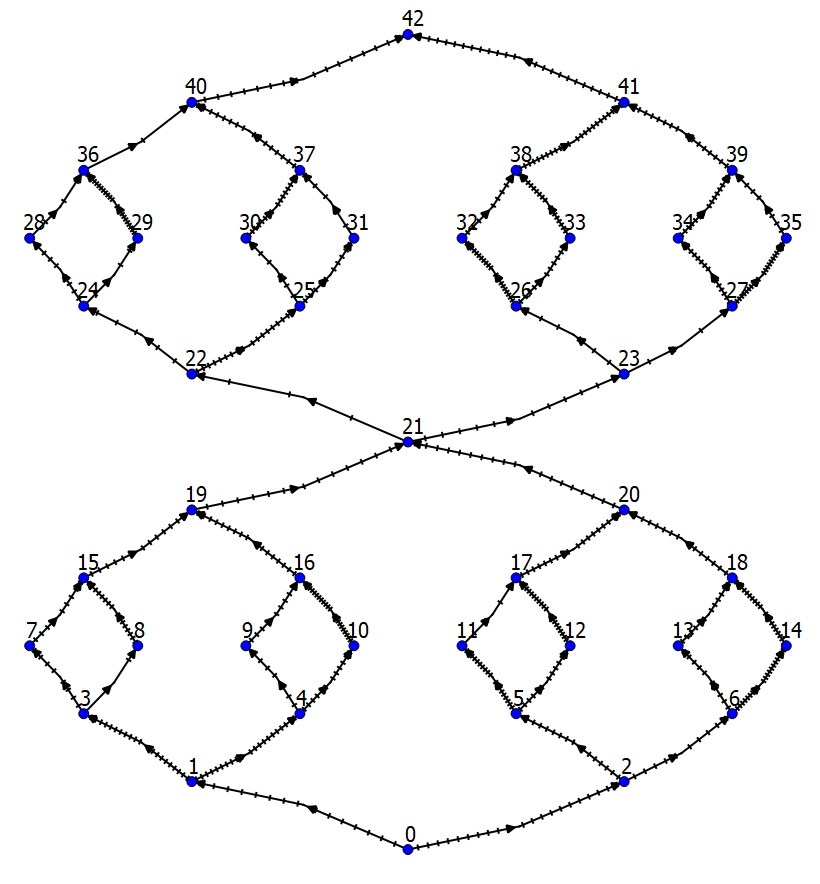
\includegraphics[scale=0.2]{graph_example.jpg}
	\caption{Граф дорожной сети $G$, на котором производилось моделирование движения. $|V| = 43, \; |E| = 52$, ребра произвольной длины. Одно деление на ребре соответствует расстоянию $L = 500$).}
	\label{ris:graph_example}
\end{figure}

Случайным образом запустим $n = 50$ участников из вершины с номером 0 в вершину с номером 42.
Выбор такого графа обусловлен тем, что в нем имеются участики сужения и расширения, которые позволят в полной мере исследовать результат взаимодействия участников.

Для того, чтобы обеспечить между участниками некоторое расстояние в начальный момент времени, запустим их с промежутками в $\Delta t = 0.2$.

Предположим, что в некоторый момент времени $t_{st}$ из вершины с номером 0 выезжает участник в вершину с номером 42. Рассмотрим две модели движения АТС: модель следования за лидером (см. рис. \ref{ris:micro_diag}) и макроскопическую модель \eqref{eq:example_macro}. Исследуем возможность применения модифицированного алгоритма Дейкстры к задаче оптимизации маршрута путем сравнения с обычным перебором (см. таблицы \ref{tab:res_micro_dep}, \ref{tab:res_micro_indep}, \ref{tab:res_macro_dep}, \ref{tab:res_macro_indep},). 

\begin{table}[H]
	\tiny
	\caption{Результаты запуска программы поиска оптимального пути в микроскопической модели следования за лидером при условии влияния добавленного участника на движение остальных в зависимости от параметров  $v_{max}, \; v_{min}, \; a$, где $a = \frac{v^2_{max}-v^2_{min}}{2(D-l)}$.}
	\begin{tabular}{|c|c|c|c|c|c|c|l|c|c|l|c|c|}
	\hline
	&                          &                             &                             &                       & \multicolumn{3}{c|}{Перебор}                                                                                                                & \multicolumn{3}{c|}{Мод. Дейкстра}                                                                                                          &                                 &                                 \\ \cline{6-11}
	\multirow{-2}{*}{} & \multirow{-2}{*}{$t_{st}$} & \multirow{-2}{*}{$v_{max}$} & \multirow{-2}{*}{$v_{min}$} & \multirow{-2}{*}{$a$} & $T(p^*)$ & \begin{tabular}[c]{@{}c@{}}Кол-во итераций\\ моделирования\end{tabular} & \begin{tabular}[c]{@{}l@{}}Время\\ работы, с\end{tabular} & $T(p^*)$ & \begin{tabular}[c]{@{}c@{}}Кол-во итераций\\ моделирования\end{tabular} & \begin{tabular}[c]{@{}l@{}}Время\\ работы, с\end{tabular} & \multirow{-2}{*}{$\min\limits_{p} T(p)$} & \multirow{-2}{*}{$\max\limits_{p} T(p)$} \\ \hline
	1                  & 5                                                  & 60                          & 10                          & 4.375                 & 1129.16  & 64                                                                      & 16.7008                                                & 1129.16  & 52                                                                      & 12.3305                                                & 1129.16                         & 2018.37                         \\ \hline
	2                  & 5                                                  & 60                          & 20                          & 4                     & 1114.88  & 64                                                                      & 27.197                                                 & 1114.88  & 52                                                                      & 30.4414                                                & 1114.88                         & 1967.52                         \\ \hline
	3                  & 5                                                  & 80                          & 10                          & 7.875                 & 850.046  & 64                                                                      & 19.2823                                                & 850.046  & 52                                                                      & 12.4218                                                & 850.046                         & 1471.65                         \\ \hline
	4                  & 5                                                  & 80                          & 20                          & 7.5                   & 841.158  & 64                                                                      & 14.2945                                                & 841.158  & 52                                                                      & 15.3071                                                & 841.158                         & 1470.66                         \\ \hline
	5                  & 40                                                 & 60                          & 10                          & 4.375                 & 1273.21  & 64                                                                      & 23.071                                                 & 1273.21  & 52                                                                      & 12.226                                                 & 1273.21                         & 2151.37                         \\ \hline
	6                  & 40                                                 & 60                          & 20                          & 4                     & 1231.54  & 64                                                                      & 27.1132                                                & 1231.54  & 52                                                                      & 34.6609                                                & 1231.54                         & 2101.94                         \\ \hline
	7                  & 40                                                 & 80                          & 10                          & 7.875                 & 971.713  & 64                                                                      & 19.0107                                                & 971.713  & 51                                                                      & 13.8246                                                & 971.713                         & 1623.74                         \\ \hline
	8                  & 40                                                 & 80                          & 20                          & 7.5                   & 945.739  & 64                                                                      & 28.5323                                                & 945.739  & 52                                                                      & 34.8503                                                & 945.739                         & 1595.29                         \\ \hline
\end{tabular}
	\label{tab:res_micro_dep}
\end{table}

\begin{table}[H]
	\tiny
	\caption{Результаты запуска программы поиска оптимального пути в микроскопической модели следования за лидером при условии отсутствия влияния добавленного участника на движение остальных в зависимости от параметров  $v_{max}, \; v_{min}, \; a$, где $a = \frac{v^2_{max}-v^2_{min}}{2(D-l)}$.}
	\begin{tabular}{|c|c|c|c|c|c|c|l|c|c|l|c|c|}
		\hline
		& & & & & \multicolumn{3}{c|}{Перебор} & \multicolumn{3}{c|}{Мод. Дейкстра} & & \\ \cline{6-11}
		\multirow{-2}{*}{} & \multirow{-2}{*}{$t_{st}$} & \multirow{-2}{*}{$v_{max}$} & \multirow{-2}{*}{$v_{min}$} & \multirow{-2}{*}{$a$} & $T(p^*)$ & \begin{tabular}[c]{@{}c@{}}Кол-во итераций\\ моделирования\end{tabular} & \begin{tabular}[c]{@{}l@{}}Время\\ работы, с\end{tabular} & $T(p^*)$ & \begin{tabular}[c]{@{}c@{}}Кол-во итераций\\ моделирования\end{tabular} & \begin{tabular}[c]{@{}l@{}}Время\\ работы, с\end{tabular} & \multirow{-2}{*}{$\min\limits_{p} T(p)$} & \multirow{-2}{*}{$\max\limits_{p} T(p)$} \\ \hline
		1                 & 5                         & 60                         & 10                         & 4.375                & 1142.26  & 64                                                                      & 27.0787                                                & 1142.26  & 52                                                                      & 39.7554                                                & 1142.26                        & 2018.37                        \\ \hline
		2                 & 5                         & 60                         & 20                         & 4                    & 1114.88  & 64                                                                      & 33.0677                                                & 1114.88  & 52                                                                      & 23.0935                                                & 1114.88                        & 2014.19                        \\ \hline
		3                 & 5                         & 80                         & 10                         & 7.875                & 850.046  & 64                                                                      & 30.5048                                                & 850.046  & 52                                                                      & 17.3063                                                & 850.046                        & 1471.65                        \\ \hline
		4                 & 5                         & 80                         & 20                         & 7.5                  & 841.158  & 64                                                                      & 29.033                                                 & 841.158  & 52                                                                      & 18.1372                                                & 841.158                        & 1479.91                        \\ \hline
		5                 & 40                        & 60                         & 10                         & 4.375                & 1273.21  & 64                                                                      & 28.2584                                                & 1273.21  & 52                                                                      & 14.2799                                                & 1273.21                        & 2151.37                        \\ \hline
		6                 & 40                        & 60                         & 20                         & 4                    & 1231.54  & 64                                                                      & 36.577                                                 & 1231.54  & 52                                                                      & 20.4323                                                & 1231.54                        & 2101.94                        \\ \hline
		7                 & 40                        & 80                         & 10                         & 7.875                & 971.713  & 64                                                                      & 33.1075                                                & 971.713  & 51                                                                      & 14.571                                                 & 971.713                        & 1623.74                        \\ \hline
		8                 & 40                        & 80                         & 20                         & 7.5                  & 945.739  & 64                                                                      & 25.1396                                                & 945.739  & 52                                                                      & 20.1858                                                & 945.739                        & 1595.29                        \\ \hline
	\end{tabular}
	\label{tab:res_micro_indep}
\end{table}

\begin{table}[H]
	\tiny
	\caption{Результаты запуска программы поиска оптимального пути в макроскопической модели при условии влияния добавленного участника на движение остальных в зависимости от параметров  $v_{max}, \; v_{min}, \; a$, где $a = \frac{v^2_{max}-v^2_{min}}{2(D-l)}$.}
	\begin{tabular}{|c|c|c|c|c|c|c|l|c|c|l|c|c|}
		\hline
		& & & & & \multicolumn{3}{c|}{Перебор} & \multicolumn{3}{c|}{Мод. Дейкстра} & & \\ \cline{6-11}
		\multirow{-2}{*}{} & \multirow{-2}{*}{$t_{st}$} & \multirow{-2}{*}{$v_{max}$} & \multirow{-2}{*}{$v_{min}$} & \multirow{-2}{*}{$a$} & $T(p^*)$ & \begin{tabular}[c]{@{}c@{}}Кол-во итераций\\ моделирования\end{tabular} & \begin{tabular}[c]{@{}l@{}}Время\\ работы, с\end{tabular} & $T(p^*)$ & \begin{tabular}[c]{@{}c@{}}Кол-во итераций\\ моделирования\end{tabular} & \begin{tabular}[c]{@{}l@{}}Время\\ работы, с\end{tabular} & \multirow{-2}{*}{$\min\limits_{p} T(p)$} & \multirow{-2}{*}{$\max\limits_{p} T(p)$} \\ \hline
		1 & 5 & 60 & 10 & 4.375 & 1208.42 & 64 & 0.38878 & 1208.42 & 51 & 0.308759 & 1208.42 & 2229.88 \\ \hline
		2 & 5 & 60 & 20 & 4 & 1164.72 & 64 & 0.390943 & 1164.72 & 51 & 0.308681 & 1164.72 & 2093.01 \\ \hline
		3 & 5 & 80 & 10 & 7.875 & 914.833 & 64 & 0.389688 & 914.833 & 51 & 0.30841 & 914.833 & 1702.06 \\ \hline
		4 & 5 & 80 & 20 & 7.5 & 891.223 & 64 & 0.390798 & 891.223 & 51 & 0.307565 & 891.223 & 1617.92 \\ \hline
		5 & 40 & 60 & 10 & 4.375 & 1220.1 & 64 & 0.389539 & 1220.1 & 51 & 0.308927 & 1220.1 & 2230.95 \\ \hline
		6 & 40 & 60 & 20 & 4 & 1177.82 & 64 & 0.390696 & 1177.82 & 51 & 0.307389 & 1177.82 & 2096.77 \\ \hline
		7 & 40 & 80 & 10 & 7.875 & 926.374 & 64 & 0.394311 & 926.374 & 51 & 0.309656 & 926.374 & 1702.62 \\ \hline
		8 & 40 & 80 & 20 & 7.5 & 902.47 & 64 & 0.392885 & 902.47 & 51 & 0.308543 & 902.47 & 1620.23 \\ \hline
	\end{tabular}
	\label{tab:res_macro_dep}
\end{table}

\begin{table}[H]
	\tiny
	\caption{Результаты запуска программы поиска оптимального пути в макроскопической модели при условии отсутствия влияния добавленного участника на движение остальных в зависимости от параметров  $v_{max}, \; v_{min}, \; a$, где $a = \frac{v^2_{max}-v^2_{min}}{2(D-l)}$.}
	\begin{tabular}{|c|c|c|c|c|c|c|l|c|c|l|c|c|}
		\hline
		& & & & & \multicolumn{3}{c|}{Перебор} & \multicolumn{3}{c|}{Мод. Дейкстра} & & \\ \cline{6-11}
		\multirow{-2}{*}{} & \multirow{-2}{*}{$t_{st}$} & \multirow{-2}{*}{$v_{max}$} & \multirow{-2}{*}{$v_{min}$} & \multirow{-2}{*}{$a$} & $T(p^*)$ & \begin{tabular}[c]{@{}c@{}}Кол-во итераций\\ моделирования\end{tabular} & \begin{tabular}[c]{@{}l@{}}Время\\ работы, с\end{tabular} & $T(p^*)$ & \begin{tabular}[c]{@{}c@{}}Кол-во итераций\\ моделирования\end{tabular} & \begin{tabular}[c]{@{}l@{}}Время\\ работы, с\end{tabular} & \multirow{-2}{*}{$\min\limits_{p} T(p)$} & \multirow{-2}{*}{$\max\limits_{p} T(p)$} \\ \hline
		1 & 5 & 60 & 10 & 4.375 & 1202.6 & 64 & 0.409948 & 1202.6 & 51 & 0.309044 & 1202.6 & 2210.82 \\ \hline
		2 & 5 & 60 & 20 & 4 & 1161.61 & 64 & 0.417604 & 1161.61 & 51 & 0.309546 & 1161.61 & 2082.44 \\ \hline
		3 & 5 & 80 & 10 & 7.875 & 910.634 & 64 & 0.389438 & 910.634 & 51 & 0.311105 & 910.634 & 1685.62 \\ \hline
		4 & 5 & 80 & 20 & 7.5 & 888.15 & 64 & 0.390584 & 888.15 & 51 & 0.310151 & 888.15 & 1607.24 \\ \hline
		5 & 40 & 60 & 10 & 4.375 & 1214.21 & 64 & 0.39104 & 1214.21 & 51 & 0.30969 & 1214.21 & 2213.23 \\ \hline
		6 & 40 & 60 & 20 & 4 & 1172.99 & 64 & 0.412499 & 1172.99 & 51 & 0.310533 & 1172.99 & 2086.97 \\ \hline
		7 & 40 & 80 & 10 & 7.875 & 921.952 & 64 & 0.418656 & 921.952 & 51 & 0.312077 & 921.952 & 1687.66 \\ \hline
		8 & 40 & 80 & 20 & 7.5 & 898.244 & 64 & 0.412369 & 898.244 & 51 & 0.312483 & 898.244 & 1610.64 \\ \hline
	\end{tabular}
	\label{tab:res_macro_indep}
\end{table}

На основе полученных результатов можно сделать следующие выводы:
\begin{itemize}
\item Для обеих моделей модифицированный алгоритм Дейкстры позволяет получить оптимальный путь независимо от влияния нового участника на движения остальных, даже при условии, что неравенство прохождения ребер \eqref{eq:neravenstvo_prohojdenya} может не выполняться.

\item Макроскопическая модель требует меньших вычислительных ресурсов для моделирования по сравнению с микроскопической моделью.

\item На практике оказалось, что алгоритм Дейкстры до момента посещения точки назначения успел промоделировать передвижение по всем ребрам, быть может кроме одного.

\item Микроскопическая модель более приближена к естественному движению автомобилей, и на практике, как мы и предполагали при постановке задачи, влияние нового участника на другие АТС оказалось ничтожно мало. 


\end{itemize}

 %%макро топ
 %%Ой, а для зависимых n от n+1 вообще все другое получилось... или нет?

%Ой, а для зависимых n от n+1 вообще все другое получилось... или нет?

\if 0
\newpage
\section{Практические результаты}
Рассмотрим микроскопическую модель следования за лидером, определенную правилами, представленными на диаграмме (рис. \ref{ris:deikstra}) и промоделируем ее на графе дорожной сети $G$ (см. рис. \ref{ris:Graph}).

\begin{figure}[H]
	\centering
	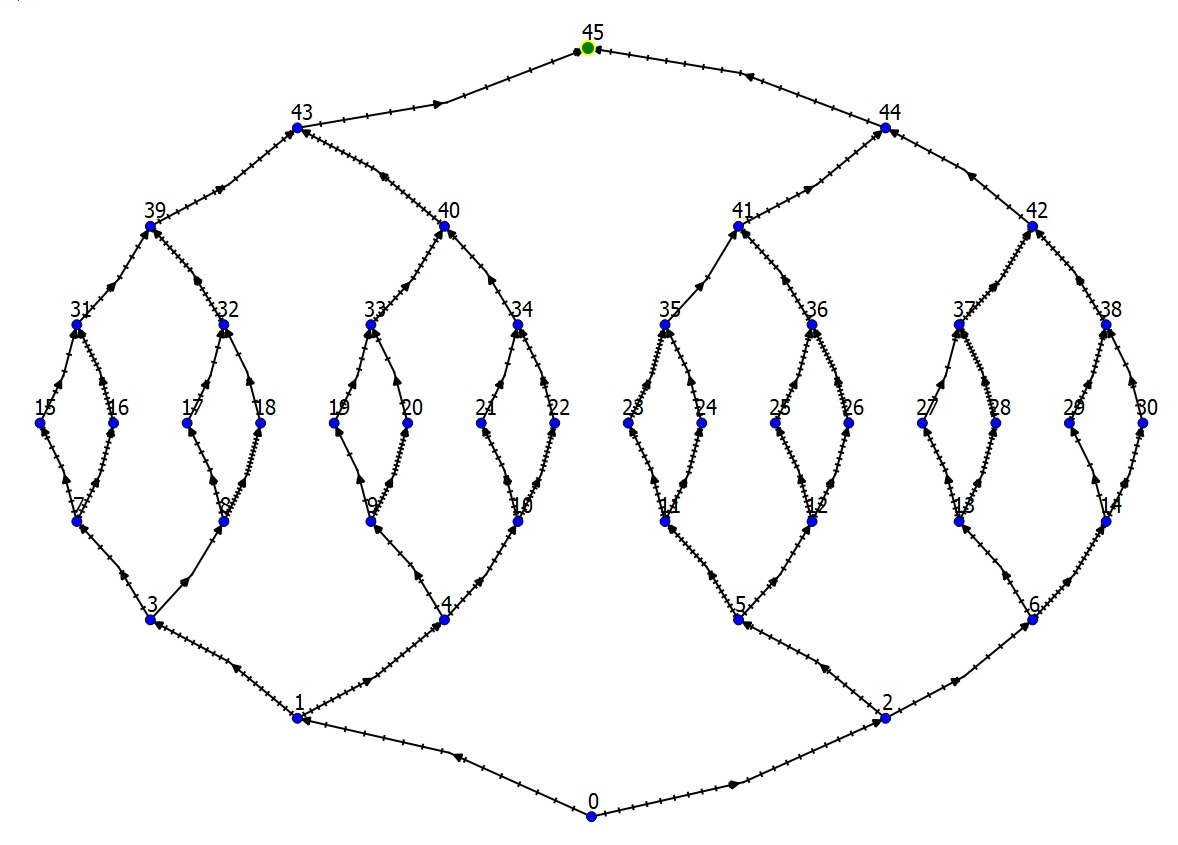
\includegraphics[scale=0.25]{Graph_N.jpg}
	\caption{Граф дорожной сети $G$, на котором производилось моделирование движения. $|V| = 46, \; |E| = 60$, ребра произвольной длины.}
	\label{ris:Graph}
\end{figure}

Запустим движение $n = 49$ участников по некоторым зафиксированным путям $p_1, \dots, p_{49}$, ведущим из $0$-ой в $45$-ую вершину, с добавлением $50$-ого участника с теми же концевыми вершинами. Положим $D = 500, \; l = 100, \; a = \frac{v^2_{max}-v^2_{min}}{2(D-l)}$ --- такое ускорение, которое позволяет разогнаться с $v_{min}$ до $v_{max}$ и оказаться на безопасном расстоянии $D$ до лидера, пройдя расстояние $D-l$. Для нахождения оптимального пути $p^*$ и времени, потраченного на его прохождение $T(p^*)$, будем использовать модифицированный алгоритм Дейкстры. В зависимости от времени старта $t_{st}$, максимальной и минимальной скоростей $v_{max}$ и $v_{min}$ были получены результаты:

\begin{table}[H]
	\label{tab:res_average}
	\centering
	\begin{tabular}{|c|c|c|c|c|}
		\hline
		\multicolumn{1}{|c|}{ $t_{st}$} & $v_{max}$  & $v_{min}$ & $a$ &  $T(p^*)$ \\ \hline
		\multicolumn{1}{|c|}{$5$}       & 60         & 10        & 4.375 &   955.321         \\ \hline
		\multicolumn{1}{|c|}{$5$}       & 60         & 20        &  4   &     935.259        \\ \hline
		\multicolumn{1}{|c|}{$5$ }      & 80         & 10        &  7.875   &    716.872         \\ \hline
		\multicolumn{1}{|c|}{$5$}       & 80 & 20                  & 7.5 &        707.094           \\ \hline
		\multicolumn{1}{|c|}{$40$}      & 60 & 10                  & 4.375    &  1172.52            \\ \hline
		\multicolumn{1}{|c|}{$40$ }     & 60 & 20                  & 4   &       1083       \\ \hline
		\multicolumn{1}{|c|}{$40$}      & 80 & 10                  & 7.875    &    906.91          \\ \hline
		\multicolumn{1}{|c|}{$40$ }     & 80 & 20                  & 7.5   &       864.625       \\ \hline
		
	\end{tabular}
	\caption{Результаты запуска модифицированного алгоритма Дейкстры. В таблце представлены значения времени на прохождение оптмального пути с параметрами $v_{max}, \; v_{min}, \; a = \frac{v^2_{max}-v^2_{min}}{2(D-l)}$.}
\end{table}

\fi
\newpage
\section*{Заключение}

В ходе написания дипломной работы были совершены следующие шаги:

\begin{itemize}
	\item Предложена автоматная форма определения модели движения АТС.
	\item Разработан и реализован алгоритм симуляции движения АТС в соответствии с заданной моделью движения.
	\item Сформулировано необходимое условие, при котором модифицированный алгоритм Дейкстры приводит к нахождению оптимального решения.
	\item Показано, что для модели следования за лидером возможно отклонение найденного решения от оптимального.
\end{itemize}

Исследование может иметь продолжение в различных направлениях: разработки более сложной и приближенной к реальности модели движения; рассмотрение случая, когда добавленный участник влияет на движение всех остальных АТС; проверки устойчивости найденного решения; поиска аналогий задачи или подзадач в разных областях математики.
\newpage
\begin{thebibliography}{0}
	
	\addcontentsline{toc}{section}{Литература}
	
	\bibitem{hydro_1} \textit{Lighthill M. J., Whitham G. B.} On kinematic waves: II. Theory of traffic
	flow on long crowded roads // Proc. R. Soc. London, Ser. A. 1955.
	V. 229. P. 281–345.
	
	\bibitem{hydro_2} \textit{Richards P. I.} Shock Waves on the Highway // Oper. Res. 1956. V. 4.
	P. 42–51.
	
	\bibitem{Tanaka} \textit{Иносэ Х., Хамада Т.} Управление дорожным движением. М.: Транс-
	порт, 1983.
	
	\bibitem{Newwell} \textit{Newell G. F.} Nonlinear effects in the dynamics of car – following //
	Oper. Res. 1961. V. 9. P. 209–229.
	
	\bibitem{book} \textit{А.\,И.~Гасников} ``Введение в математическое моделирование транспортных потоков'' --- Издательство МЦНМО --- 2013. --- 427 с.
	
	\bibitem{automat_baza} \textit{Nagel K., Schreckenberg M.} A cellular automation model for freeway
	traffic // Phys. I France. 1992. V. 2. P. 2221–2229.
	
	\bibitem{automat_phyz} \textit{Chowdhury D., Santen L., Schadschneider A.} Statistical physics of vehicular
	traffic and some related systems // Phys. Rep. 2000. V. 329.
	P. 199–329.
	
	\bibitem{automat_jam} \textit{Nagatani T.} The physics of traffic jams // Reports on Progress in Physics.
	2002. V. 65. P. 1331–1386.
	
\end{thebibliography} 

\end{document}